\documentclass{article}

% if you need to pass options to natbib, use, e.g.:
% \PassOptionsToPackage{numbers, compress}{natbib}
% before loading nips_2016
%
% to avoid loading the natbib package, add option nonatbib:
% \usepackage[nonatbib]{nips_2016}

\usepackage[final, nonatbib]{nips_2016}

% to compile a camera-ready version, add the [final] option, e.g.:
% \usepackage[final]{nips_2016}

\usepackage[utf8]{inputenc} % allow utf-8 input
\usepackage[T1]{fontenc}    % use 8-bit T1 fonts
\usepackage{hyperref}       % hyperlinks
\usepackage{url}            % simple URL typesetting
\usepackage{booktabs}       % professional-quality tables
\usepackage{amsfonts, amssymb, amsmath}       % blackboard math symbols
\usepackage{nicefrac}       % compact symbols for 1/2, etc.
\usepackage{microtype}      % microtypography
\usepackage{graphicx}
\usepackage{algpseudocode}
\usepackage{algorithmicx}
\usepackage{csvsimple}
\usepackage{subcaption}


\newcommand{\bX}{\mathbf{X}}
\newcommand{\bY}{\mathbf{Y}}
\newcommand{\bbeta}{\mathbf{\beta}}



\graphicspath{ {images/} }

\title{Survival of the Fittest: Variable Selection on Galapagos Agricultural Data}

\author{
  Michael Bostwick\\
  Department of Statistics and Operations Research\\
  University of North Carolina at Chapel Hill\\
	\\
  \bf{Client: Francisco Laso} \\
  Department of Geography \\
  University of North Carolina at Chapel Hill\\
  \\
  March 8th, 2018 \\
}

\begin{document}

\maketitle
\begin{abstract}
  This paper...
  
  \end{abstract}

\section{Introduction}

\subsection{Background}

The Galapagos Islands make for a feasible and significant case study of complex systems. Due to its relative isolation and smaller size the interaction of factors can more realistically be modeled for the Galapagos Islands than other systems. Yet the Galapagos Islands also represents an important example of the competing forces of resource conservation and economic development in a rapidly changing environment. Prior work has created agent-based models of the Galapagos, but with limited interaction parameters between agents, particularly in regards to farm success walsh. In order to create a more detailed, and perhaps more accurate, simulation, the relationships between different factors on the island must be better understood. This work aims to sort through a large number of possible relationships and clarify the empirically most significant ones for future study and incorporation into simulations. 

\subsection{Data}

The data available to study the dynamics between agricultural measures and related factors primarily 
comes from the Censo de las Unidades de Producci\'on Agropecuaria (upa) de Gal\'apagos (Census of Agricultural Production 
Units (UPA) of Galapagos) ref census. This is a self-reported survey with data from 755 
farms detailing the production and sale of crops and livestock, agricultural expenses, and land use 
decisions. The response rate for this was ??. In addition to the census, data is also available from ... including information on water, energy and road access.

categories...

In total, under the direction of the client 239 variables were selected for consideration in modeling 
relationships between predictors and five outcome variables of interest. Some of the five outcome variables of interest come 
directly from survey responses, while others were derived from a combination of multiple variables. When modeling derived 
outcome variables all variables used in its calculation were removed from consideration. The client also denoted specific 
predictor variables to exclude from particular models when their inclusion would not be beneficial. For example, while the 
amount of crops sold in pounds was not directly used to calculate net income, the obvious relationship existent precluded it 
from inclusion. In addition, predictor variables that met one or more of the following criteria were removed prior to modeling: 
zero variance, extremely high (>0.99) or perfect correlation with other predictor variables, or linear dependence with other 
predictor variables (that is, two or more predictor variables could be linearly combined to create another predictor variable). The 
exact number of predictor variables included in each model varied slightly, but there were approximately 200 predictors variables examined for each model after the preceding steps were taken.

\subsection{Organization of Report}

The remainder of this report is divided into four sections, Section 2: Modeling, Section 3: Results, Section 4: Statistical 
Methods, and Section 5: Limitations and Future Work. Section 2 provides an brief overview of the analysis so that the results can be understood. In Section 3 results for each of the 5 outcome variables is provided, where standard tables and graphs are repeated for each. A more in-depth explanation of the statistical methods used is contained in Section 4, but this section can be referenced as needed. Section 5 details important considerations when interpreting the results and suggests possible avenues for future work. Lastly, References and the Appendix, including additional tables and figures, can be found at the end.

\section{Modeling}
\subsection{Challenges to address}

The primary challenge in this analysis is the vast amount of potential predictor variables. This challenge is twofold; 1.) when 
the number of predictors is large the calculation of a reliable model is difficult and 2.) interpreting the coefficients of many 
predictors simultaneously is not an easy task for humans (and will make resulting simulations overly complicated). For this 
reason, the analysis focuses on the use of two variable selection techniques that aim to build a linear model with a subset of 
the available variables that still maintains a strong explanatory/predictive performance.

Secondarily, when performing standard linear regression the error is assumed to be normally 
distributed, which means the outcome variable should be roughly normally distributed. When this is not true, as is the case for 
several outcome variables in this study, a poorly fitting model will be found with unreliable coefficients. In order to address this 
issue transformations to the data and modifications to the standard linear model will be considered.

\subsection{Overview of methods}

A brief overview of the statistical methods used is presented here to allow for understanding of results, 
but for further details see Section refstatmethods Statistical Methods. For each of the outcome variables of interest 
we build a set of linear models using the appropriate subset of predictors. Each relationship is modeled 
using Forward Selection and ElasticNet regression. Forward Selection fits a linear model by progressively adding variables to 
the model until a best fit is found. This results in only some of the variables being included, chosen in a discrete manner. 
ElasticNet regression fits a linear model by limiting the size of the coefficients so that they are smaller than in standard least 
squares, and for many variables actually shrunken to zero. Similar to Forward Selection this results in a smaller model, but 
variable selection can be carefully tuned as optimization is done in a more continuous way. In general, these techniques have 
slightly different aims. Forward Selection chooses a model that best explains the variance in the dataset at hand. Elasticnet 
chooses a model that can best make predictions on new data. Depending on the goals of analysis, one technique is not 
necessarily better so we do not compare the two quantitatively, but instead offer both results as varying perspectives on 
variable selection. While a variable being chosen by both methods provides stronger evidence that an important relationship exists, disagreement should suggest exploring both possibilities instead of one method necessarily being incorrect.

\section{Results}

\subsection{Farm Success}

The first three outcome variables of interest can be grouped together under the category of farm success; labeled as 
productivity, net income and number of workers supported. Productivity is calculated as the total pounds of crops and livestock 
produced divided by the farm surface area. Net income is calculated as the the earnings from all products 
sold minus total expenses. Number of workers supported is calculated as the total labor expenditures divided by a standard 
full-time worker's salary.

\subsubsection{Productivity}

\begin{figure}[h]
\centering
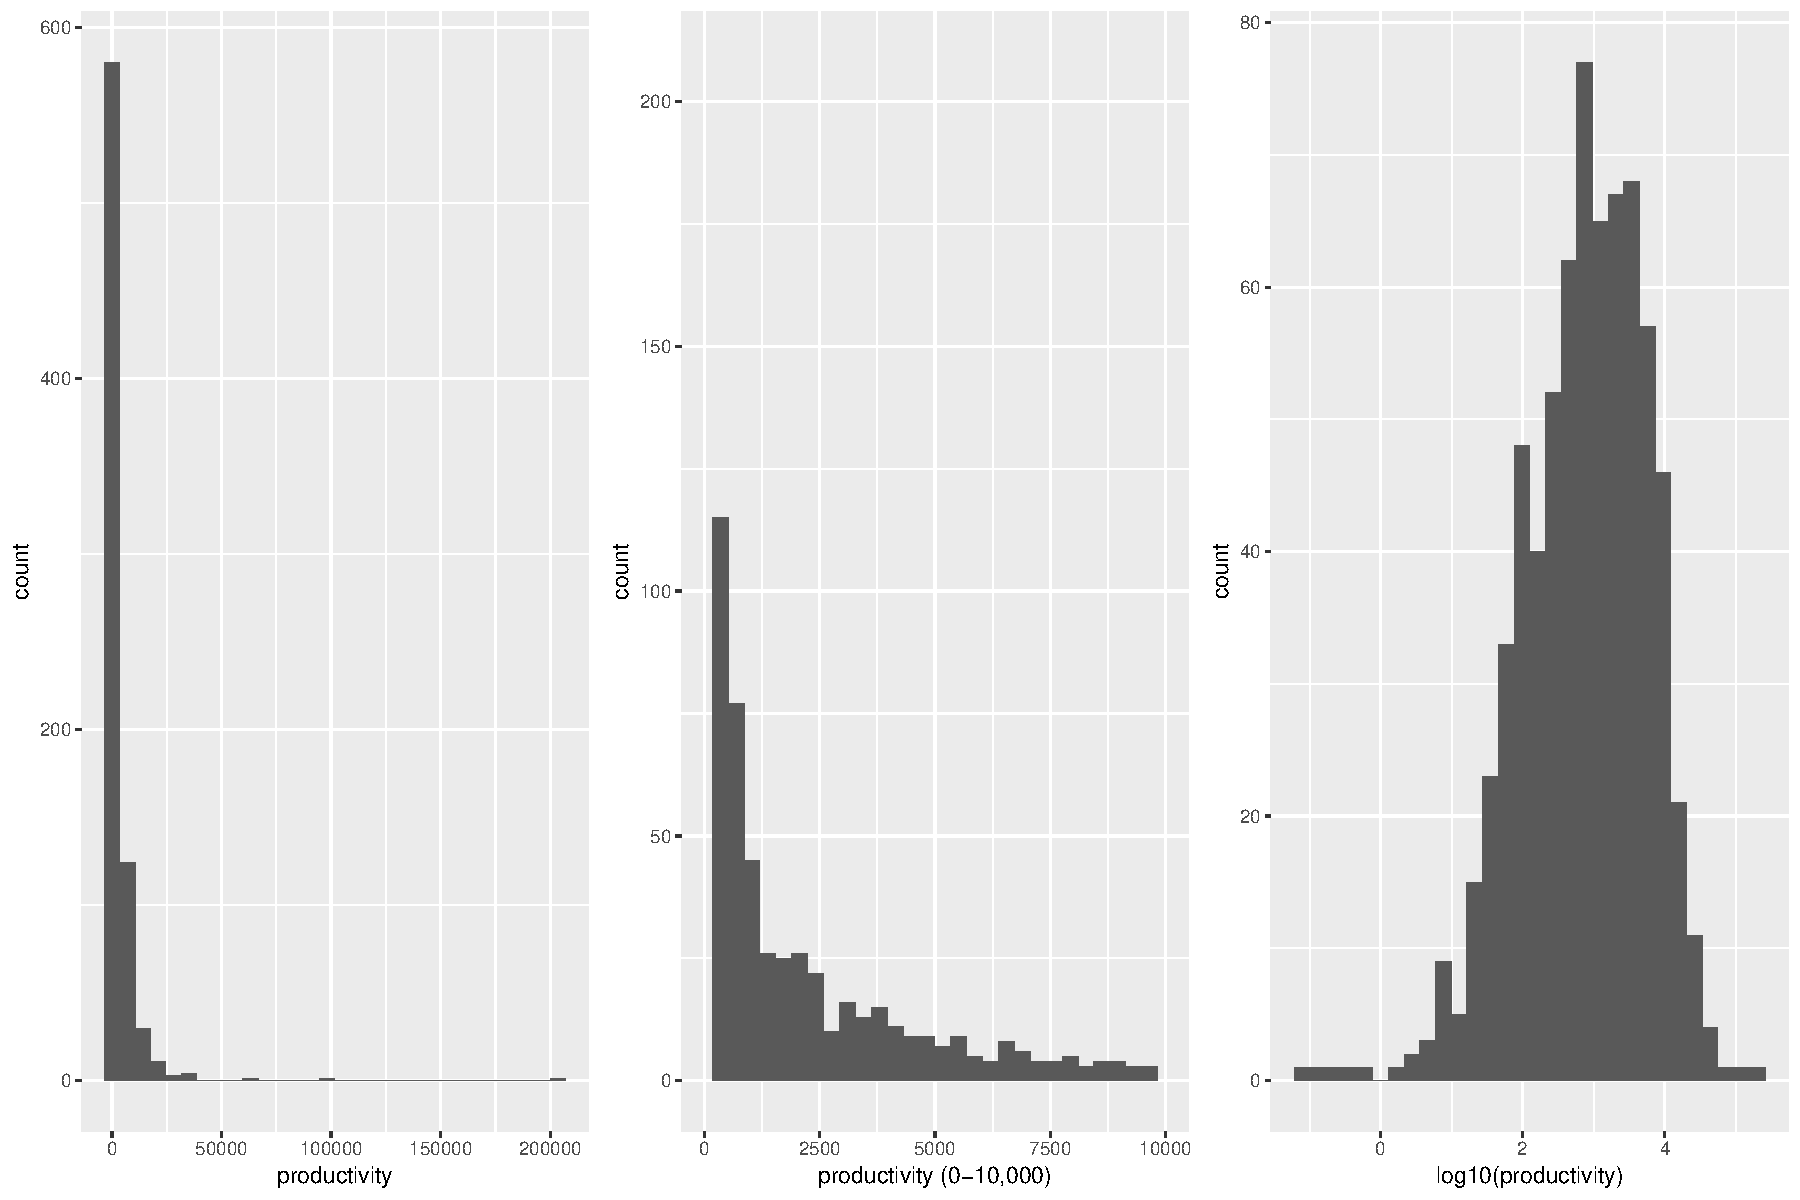
\includegraphics[width = 0.8\textwidth]{production_histograms.pdf}
\caption{Histogram of Productivity...}
\label{figure:prod_hist}
\end{figure}

The histograms of the Productivity variable (Figure \ref{figure:prod_hist}) show a strong skewness, both when looking at all 
observations, and when zooming into observations between 0-10,000 lbs/hectare. To achieve a distribution closer to normal 
(bell-curved), which will benefit the linear model, we take the $log_{10}$ transformation with resulting data shown in the last 
plot. Since the log transformation cannot be performed on zero values, we remove the ?? occasions of this from the dataset. 
Beyond the mathematical constraint, farms with zero production perhaps are not farms as typically defined.

\begin{table}[h!]
\centering
\begin{tabular}{lc|cl}\hline%
\bfseries \underline{Elasticnet} & \bfseries \underline{Forward~Selection} 
\csvreader[head to column names]{production_top5names.csv}{}%
{\\\elasticnet & \forward}%
\\\hline
\end{tabular}
\caption{Modeling of Productivity, Top 5 features for each of the three methods}
\label{table:prod_top5}
\end{table}

We build linear models using both methods, Elasticnet and Forward Selection, on the log-transformed 
productivity variable, recording an optimal model of any size and the best 5 variable model for each. The size of 5 variables is 
chosen for its interpretability and not for any specific statistical property. The results of the best 5 variable model are shown in 
Table \ref{table:prod_top5}, listed in alphabetical order.  Next to variable names the direction of the relationship is indicated with 
a (+) or (-). There is some overlap between the variables selected by each of the methods, but also unique choices made by 
each method. The Root Mean-Squared Error (RMSE) for the 5 variable model Elasticnet model is 0.78 and the $R^2$ for 
Forward Selection is 0.48. The RMSE is on average how far the predicted value is from the actual value and $R^2$ is the 
percentage of variability in the outcome variable is explained by the model.

Plots from the optimal models for Elasticnet and Forward Selection are shown in Figure \ref{figure:prod_opt}. The cross-validation plot for Elasticnet can be understood as follows: the 
horizontal axis shows the number of variables included in the model (on top) and the corresponding lambda ($\lambda$) value 
(on the bottom), the vertical axis shows the Mean-Squared Error (MSE) represented as the red dots and surrounded by bars 
showing the standard deviation. The vertical dashed line to the left, $\lambda_{min}$, is found at the minimum MSE and the 
vertical dashed line to the right, $\lambda_{1se}$ is at the largest lambda within one standard error of the minimum. The idea 
behind $\lambda_{1se}$ is that similar error performance can be achieved with a smaller model, in this case a model with 40 
less variables. Since our goal is to select a small amount of variables, we will generally use the model found at $\lambda_{1se}
$. For Forward Selection the plot is much more straightforward, we plot the number of variables included versus the 
information criterion that we would like to minimize and mark the optimal point in red.

The convex shape of the plots highlights a common trend in variable selection; not including enough variables does not provide 
enough information, but beyond a certain point adding more variables may not be worth the added complexity. The optimal 
model chosen for Elasticnet includes 45 variables (not counting the intercept term) and using Forward Selection we choose a 
model of 26 variables, almost all of which are also included in the Elasticnet model. The coefficients estimated for both models 
can be found in Table \ref{table:prod_full} in the Appendix. For the full models the RMSE and $R^2$ are 0.61 and 0.63 
respectively. These numbers suggest that while the 5 variable model is helpful, there is a decent amount of information to be 
gained by adding more variables. Diagnostics of the linear fit of the optimal Elasticnet and Forward Selection models (plots shown in Figure \ref{figure:resids_prod} in the Appendix) do not raise any concerns. 

\begin{figure}[!tbp]
\begin{subfigure}[b]{0.5\textwidth}
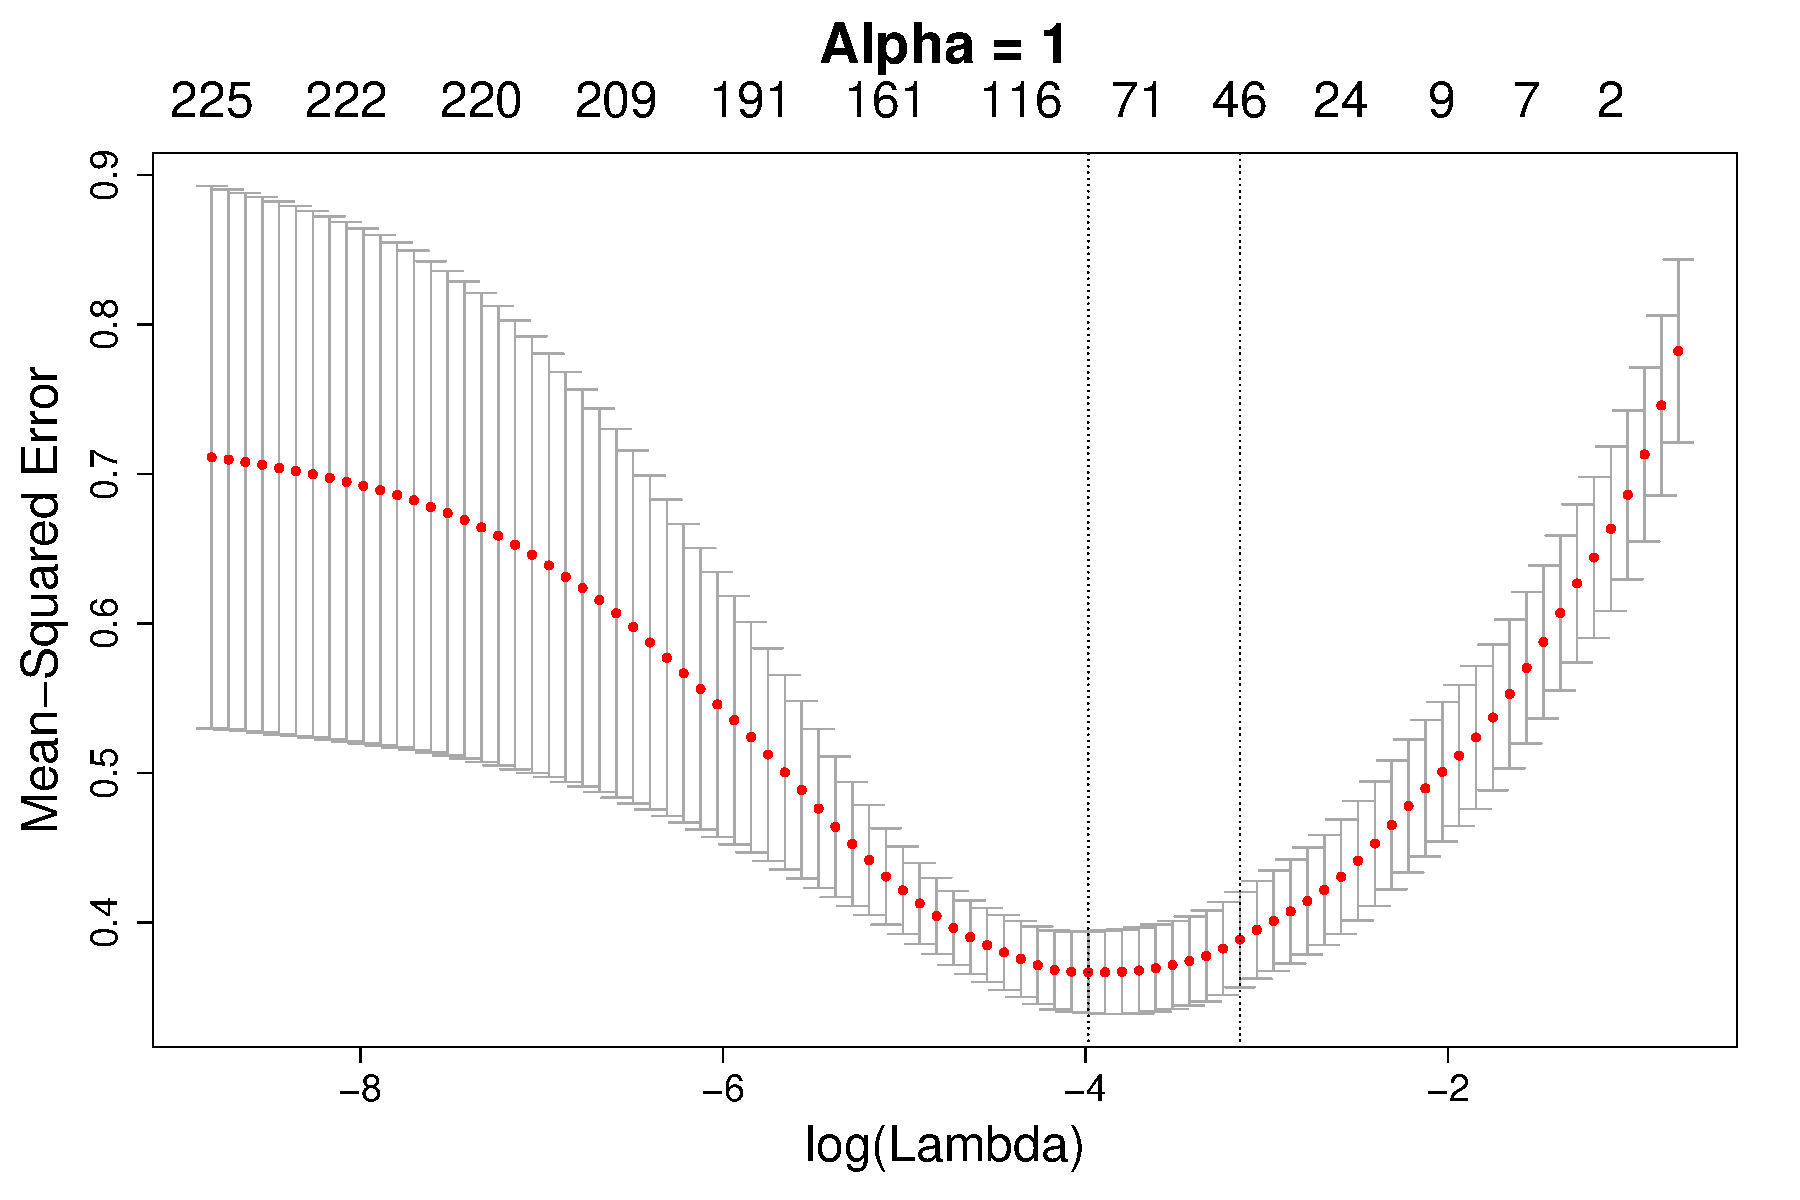
\includegraphics[width=\textwidth]{elastic_cv_production.pdf}
\caption{Cross-validation plots for Elasticnet...}
\end{subfigure}
\hfill
\begin{subfigure}[b]{0.5\textwidth}
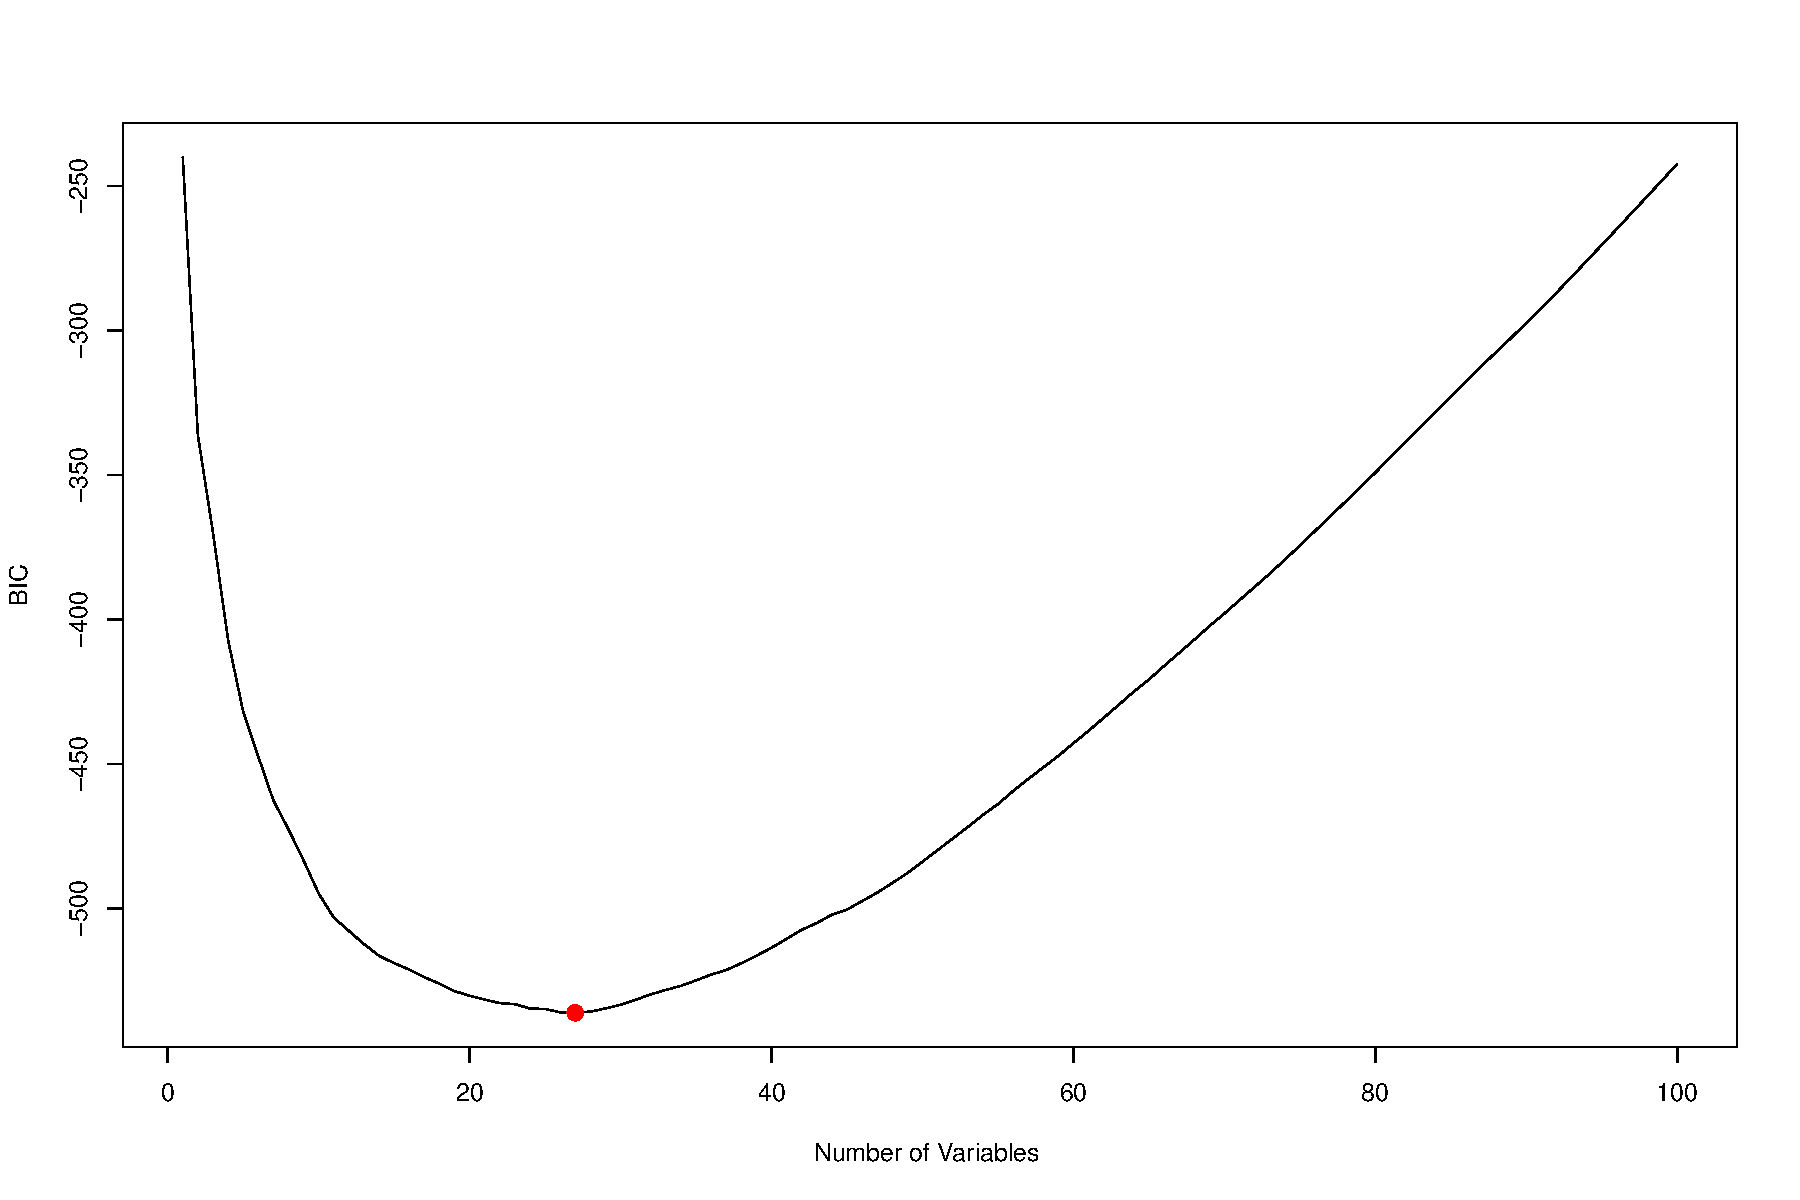
\includegraphics[width=\textwidth]{forward_nvars_production.pdf}
\caption{Number of variables Forward Selection plots...}
\end{subfigure}
\caption{Production Variable Selection}
\label{figure:prod_opt}
\end{figure}

\subsubsection{Net Income}

\begin{figure}[h]
\centering
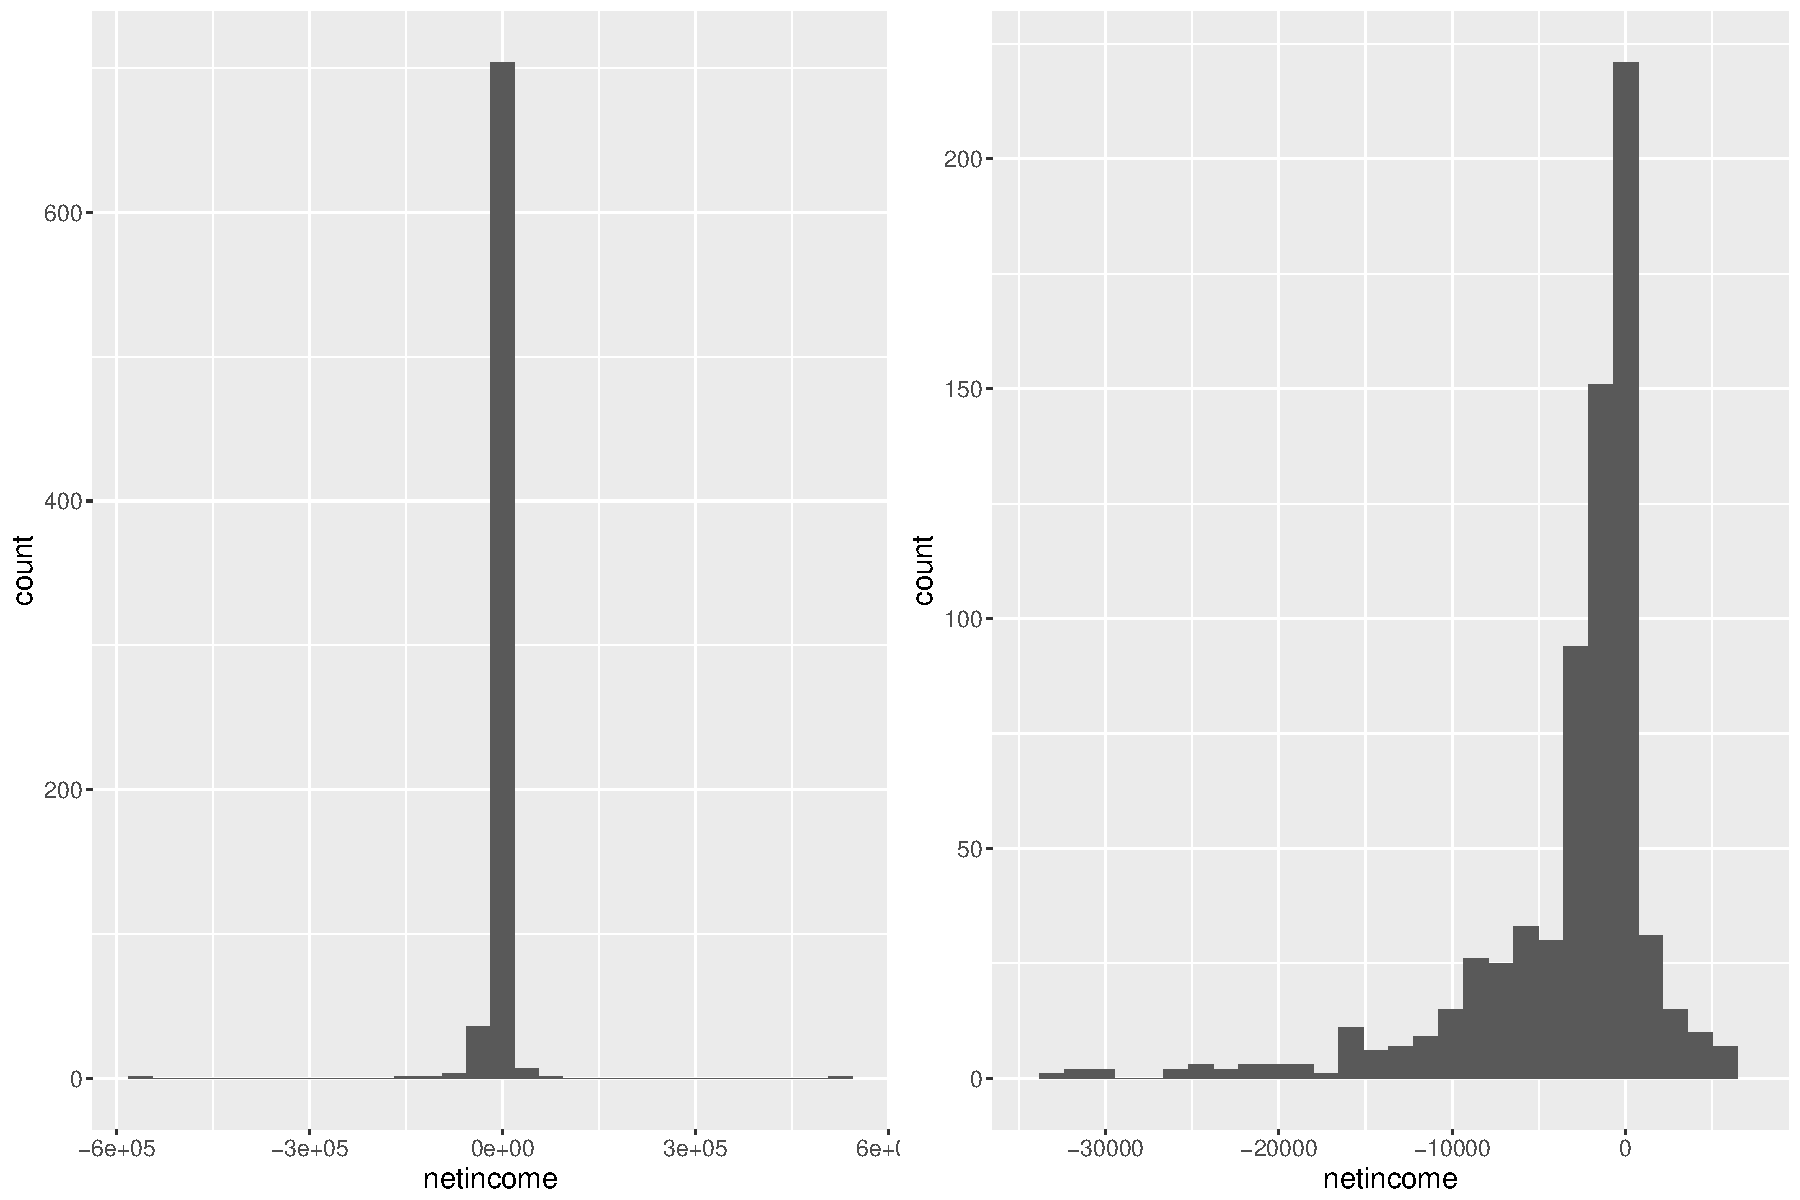
\includegraphics[width = 0.75\textwidth]{netincome_histograms.pdf}
\caption{Histogram of Net Income...}
\label{figure:netincome_hist}
\end{figure}

The histograms for Net Income (Figure \ref{figure:netincome_hist}) show a symmetric shape, but a very spiky center and a few 
observations wide in the tails. We attempt to fit a model on the full dataset, but find the observations with large absolute 
values are obscuring other possible information in the model. We then remove the 28 observations that are beyond one 
standard deviation (30,478) from the mean in either direction. The following models are fit on this reduced dataset of 727 
observations.

\begin{table}[h!]
\centering
\begin{tabular}{c|c|c}\hline%
\bfseries \underline{Elasticnet} & \bfseries \underline{Forward~Selection}
\csvreader[head to column names]{netincome_top5names.csv}{}%
{\\\elasticnet & \forward}%
\\\hline
\end{tabular}
\caption{Modeling of Net Income, Top 5 features for each of the three methods}
\label{table:netincome_top5}
\end{table}

The results of the best 5 variable model are shown in \ref{table:netincome_top5}, with a RMSE of 5790.35 for Elasticnet and a $R^2$ of 0.15 for Forward Selection. For interpretation of the RMSE it is important to keep in mind the scale for Net Income is much larger than that of log productivity.

\begin{figure}[!tbp]
\begin{subfigure}[b]{0.5\textwidth}
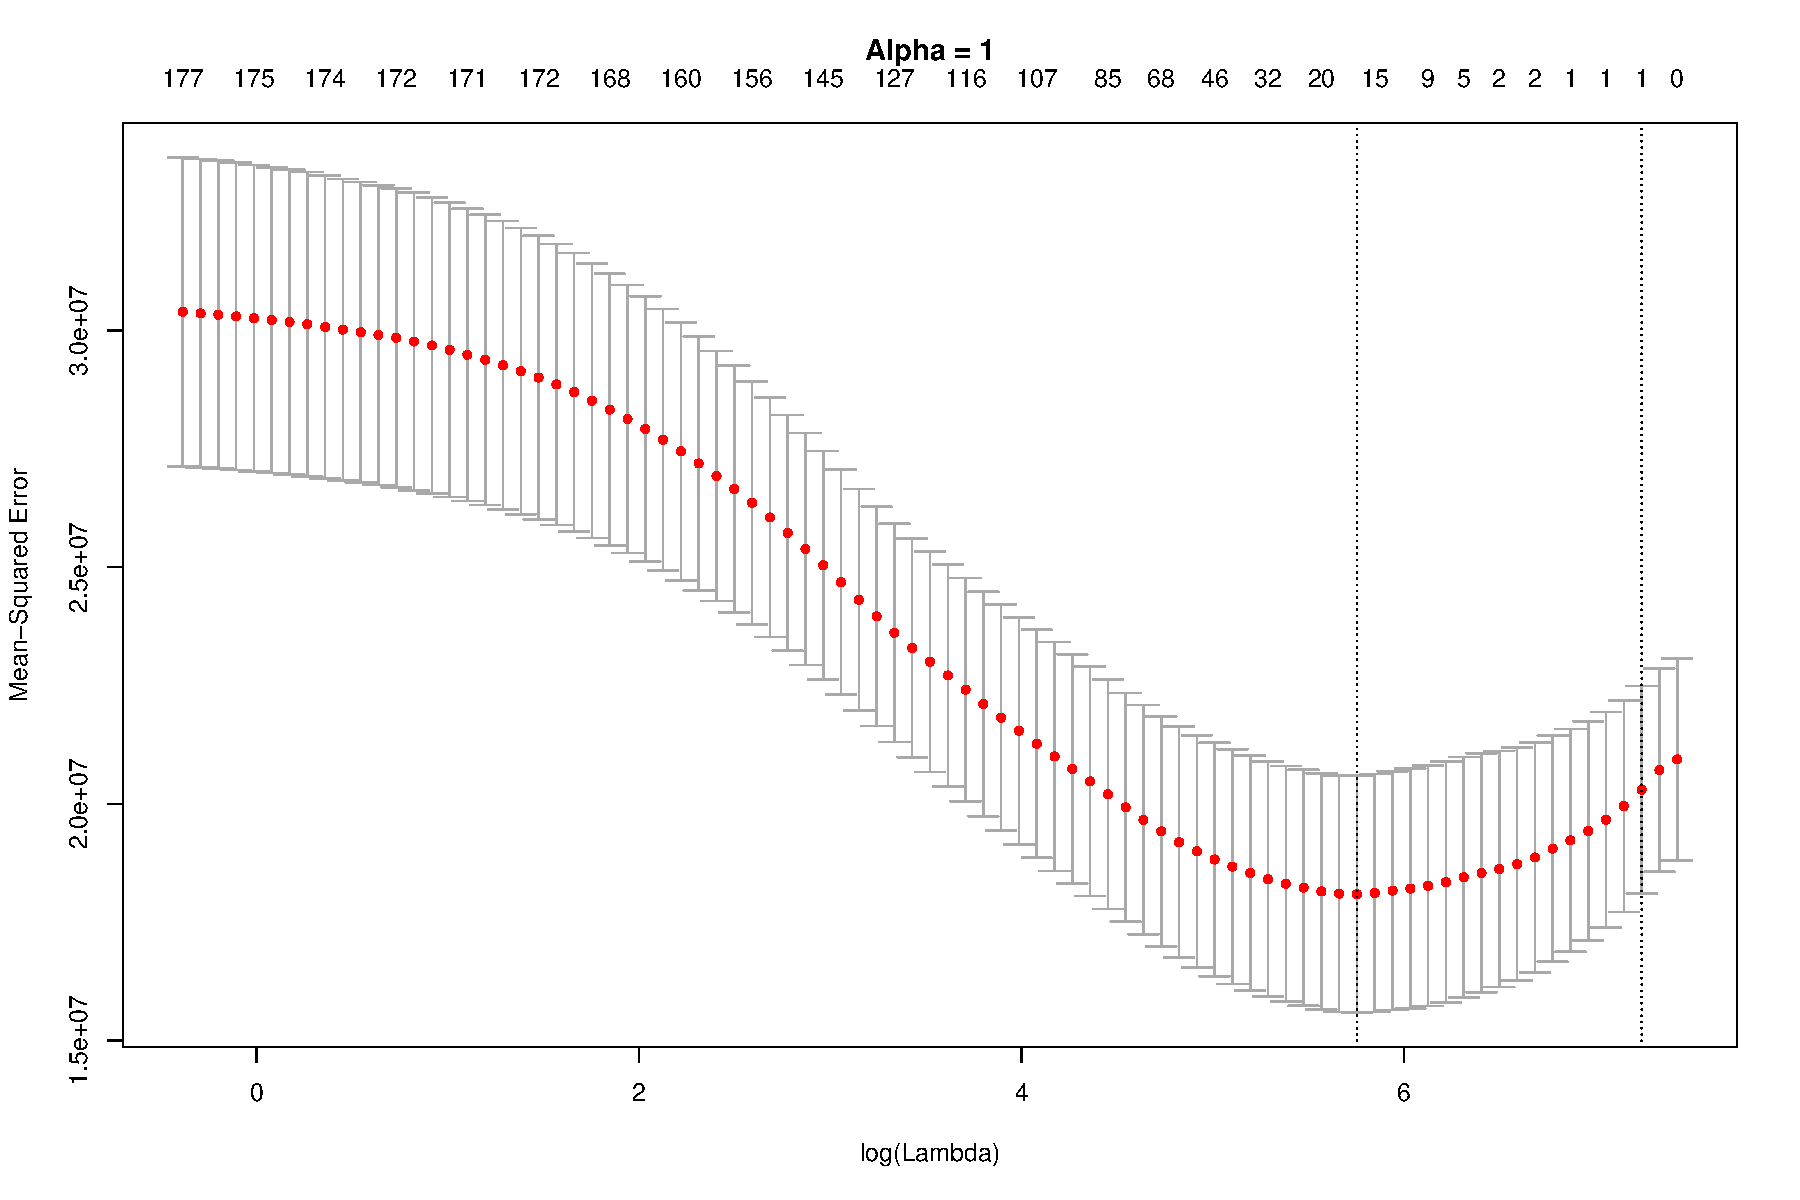
\includegraphics[width=\textwidth]{elastic_cv_netincome.pdf}
\caption{Cross-validation plots for Elasticnet...}
\end{subfigure}
\hfill
\begin{subfigure}[b]{0.5\textwidth}
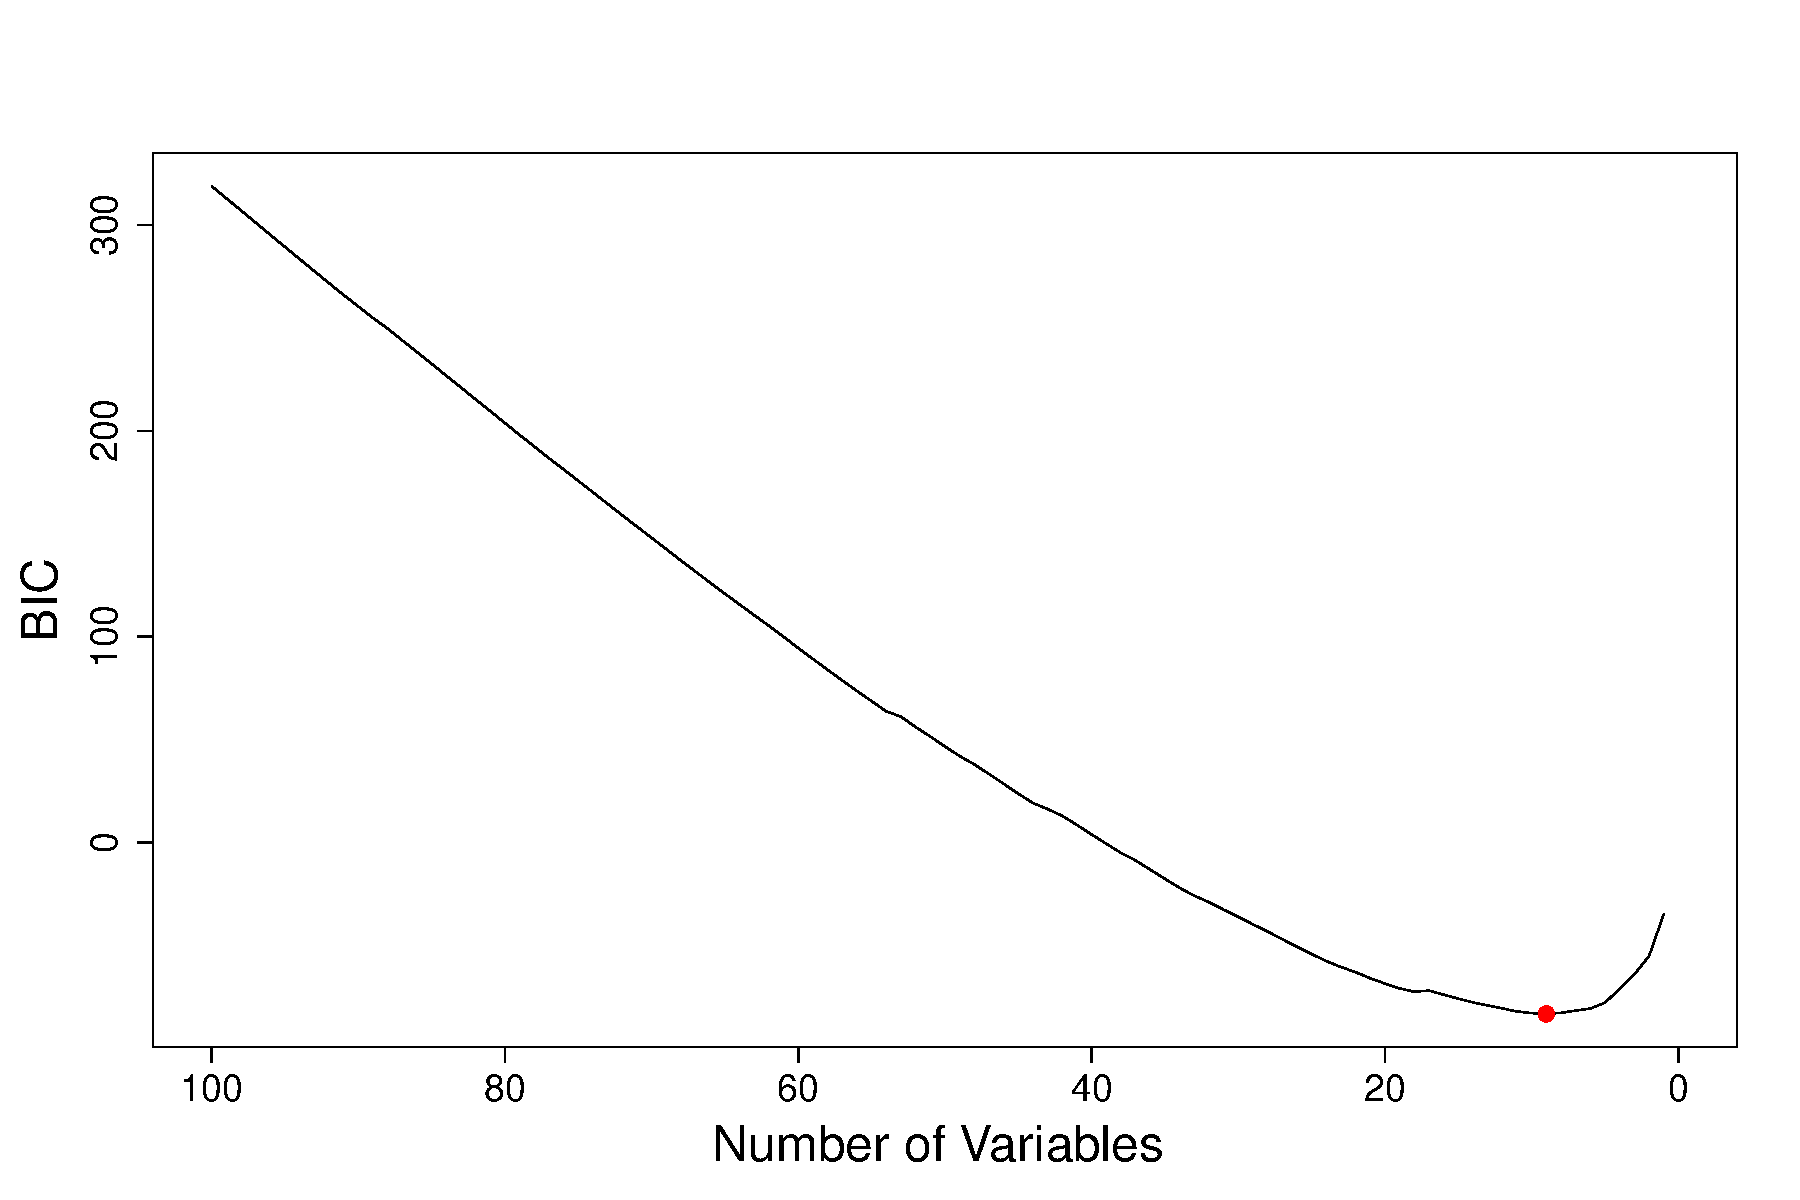
\includegraphics[width=\textwidth]{forward_nvars_netincome.pdf}
\caption{Number of variables Forward Selection plots...}
\end{subfigure}
\caption{Net Income Variable Selection}
\label{figure:netincome_opt}
\end{figure}

The cross-validation plot for Net Income show wider error bars throughout the range of model sizes and just using the average 
Net Income would predict nearly as well as any other model. Since here $\lambda_{1se}$ only includes the intercept, we 
choose the optimal Elasticnet model to be at $\lambda_{min}$, which includes 9 variables. For Forward Selection, we also 
include 9 variables, with all but two overlapping with the Elasticnet choices. The coefficents estimated for both models can be 
found in Table \ref{table:netincome_full} in the Appendix. The full models had an RMSE and $R^2$ of 5768.30 and 0.19, 
respectively. Since the full models are not much larger than the 5 variable models, the small increases are not surprising. Diagnostics of the linear fit of the optimal Elasticnet and Forward Selection models (plots shown in Figure 
\ref{figure:resids_netincome} in the Appendix) do not follow assumptions as closely as for the Production models, but are not so 
concerning as to disqualify the results. On the whole, the results from the various plots and diagnostics suggest that the relationships found for Net Income are worth investigating, but that a linear relationship is not very strong.


\subsubsection{Number of Workers Supported}

\begin{figure}[h]
\centering
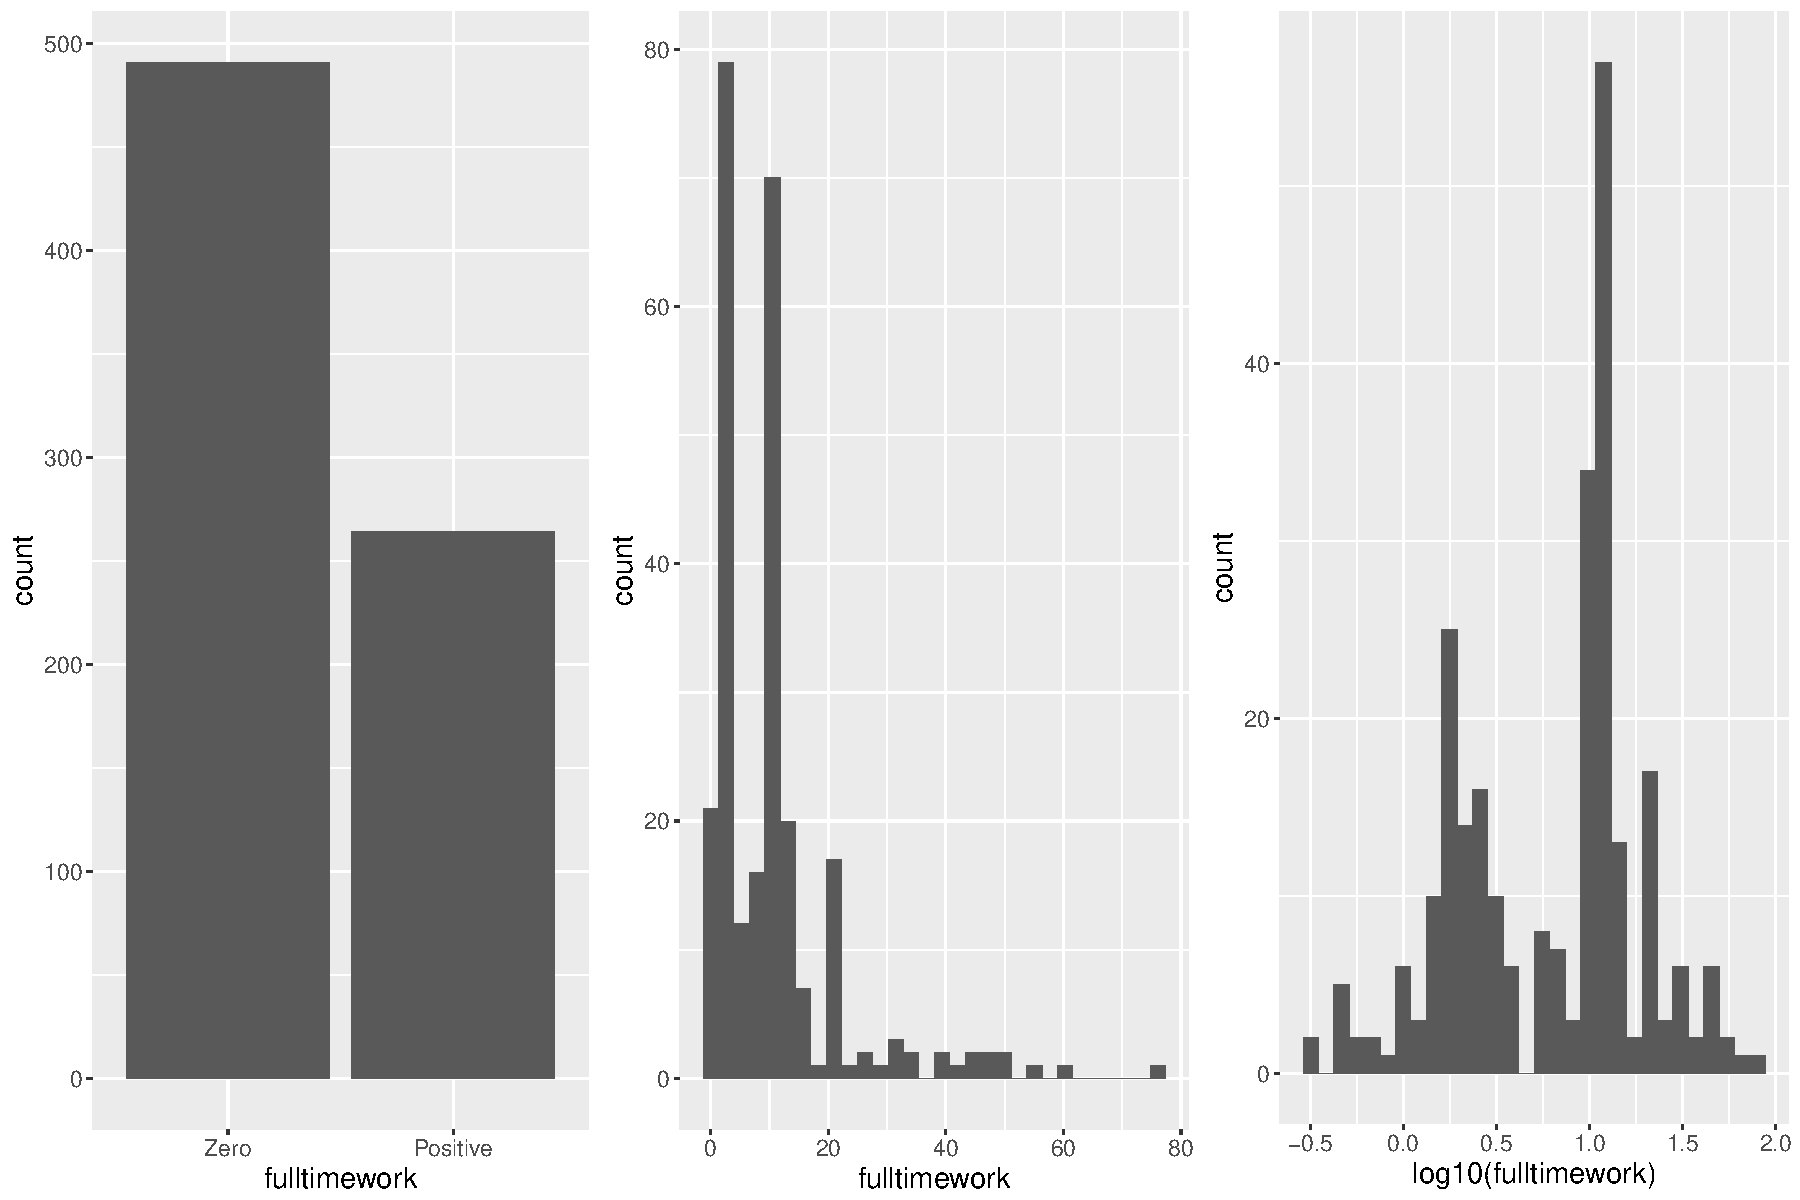
\includegraphics[width = 0.75\textwidth]{worker_histograms.pdf}
\caption{Histogram of Workers...}
\label{figure:workers_hist}
\end{figure}

The first plot in Figure \ref{figure:workers_hist} shows that a large percentage of the farms are not able to support any workers. 
For this reason, we divide up the modeling task for this outcome variable. First, we use logistic regression to model the binary 
variable of whether a farm supports more than zero or zero workers. Secondly, we use linear regression to model the quantity 
of workers for just those 264 farms with a positive number of workers supported.

\begin{table}[h]
\centering
\begin{tabular}{c|c|c}\hline%
\bfseries \underline{Elasticnet} & \bfseries \underline{Forward~Selection}
\csvreader[head to column names]{workers_binary_top5names.csv}{}%
{\\\elasticnet & \forward}%
\\\hline
\end{tabular}
\caption{Modeling of Binary Workers , Top 5 features for each method}
\label{table:workers_binary_top5}
\end{table}

\begin{table}[h!]
\centering
\begin{tabular}{c|c|c}\hline%
\bfseries \underline{Elasticnet} & \bfseries \underline{Forward~Selection}
\csvreader[head to column names]{workers_nonzero_top5names.csv}{}%
{\\\elasticnet & \forward}%
\\\hline
\end{tabular}
\caption{Modeling of Nonzero Workers , Top 5 features for each method}
\label{table:workers_nonzero_top5}
\end{table}

Sometimes Elasticnet will simultaneously choose to include multiple variables at the same time, in this case there is not a 5 
variable model so we show the 6 variable model for Elasticnet. For logistic regression we can measure performance with the 
misclassification rate, which on average is 0.31 on the test set for Elasticnet and 0.26 on the full dataset for Forward Selection. 
For the linear model 5 variable model the RMSE is 0.46 and the $R^2$  0.30. Several variables are found to be most helpful for both the logistic regression and linear regression models, but there is still a fair bit of difference.

\begin{figure}[!tbp]
\begin{subfigure}[b]{0.5\textwidth}
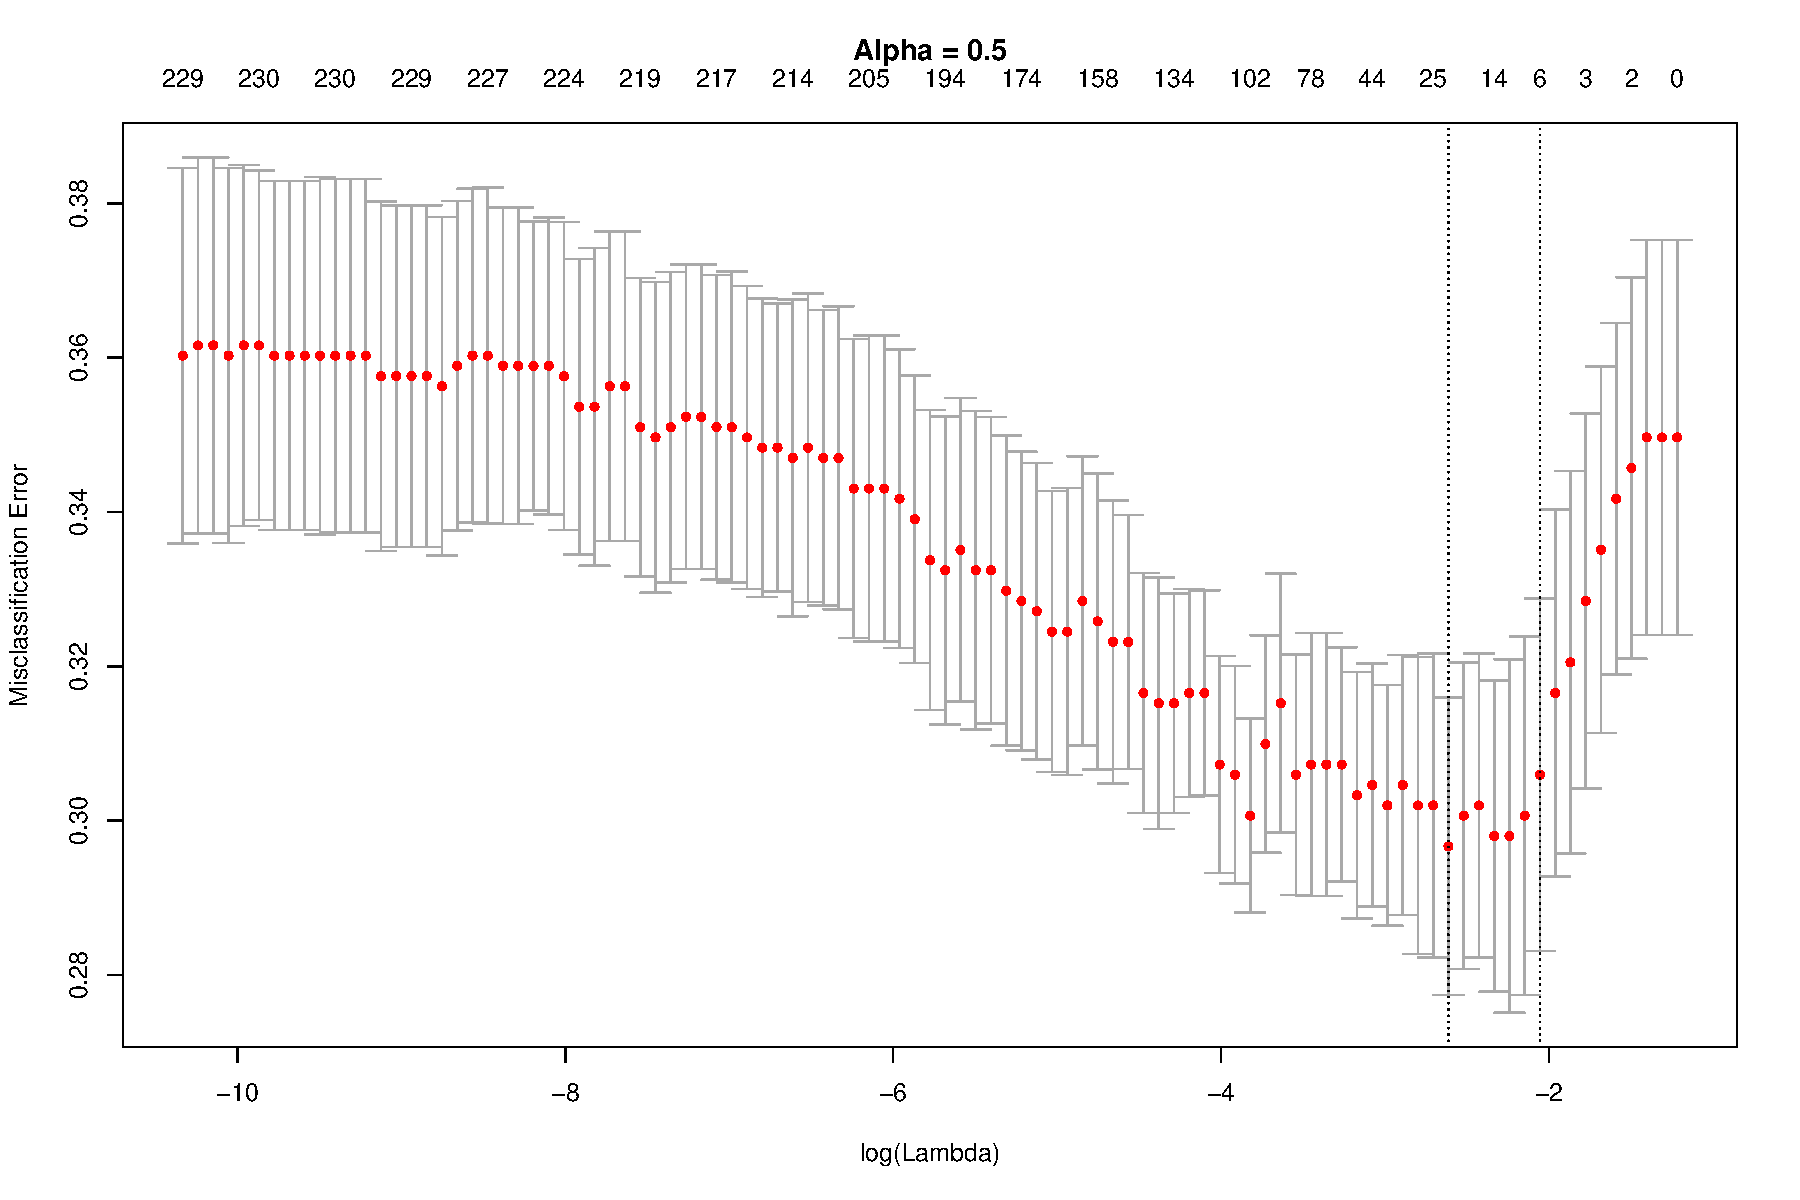
\includegraphics[width=\textwidth]{elastic_cv_workers_binary.pdf}
\caption{Cross-validation plots for Elasticnet...}
\end{subfigure}
\hfill
\begin{subfigure}[b]{0.5\textwidth}
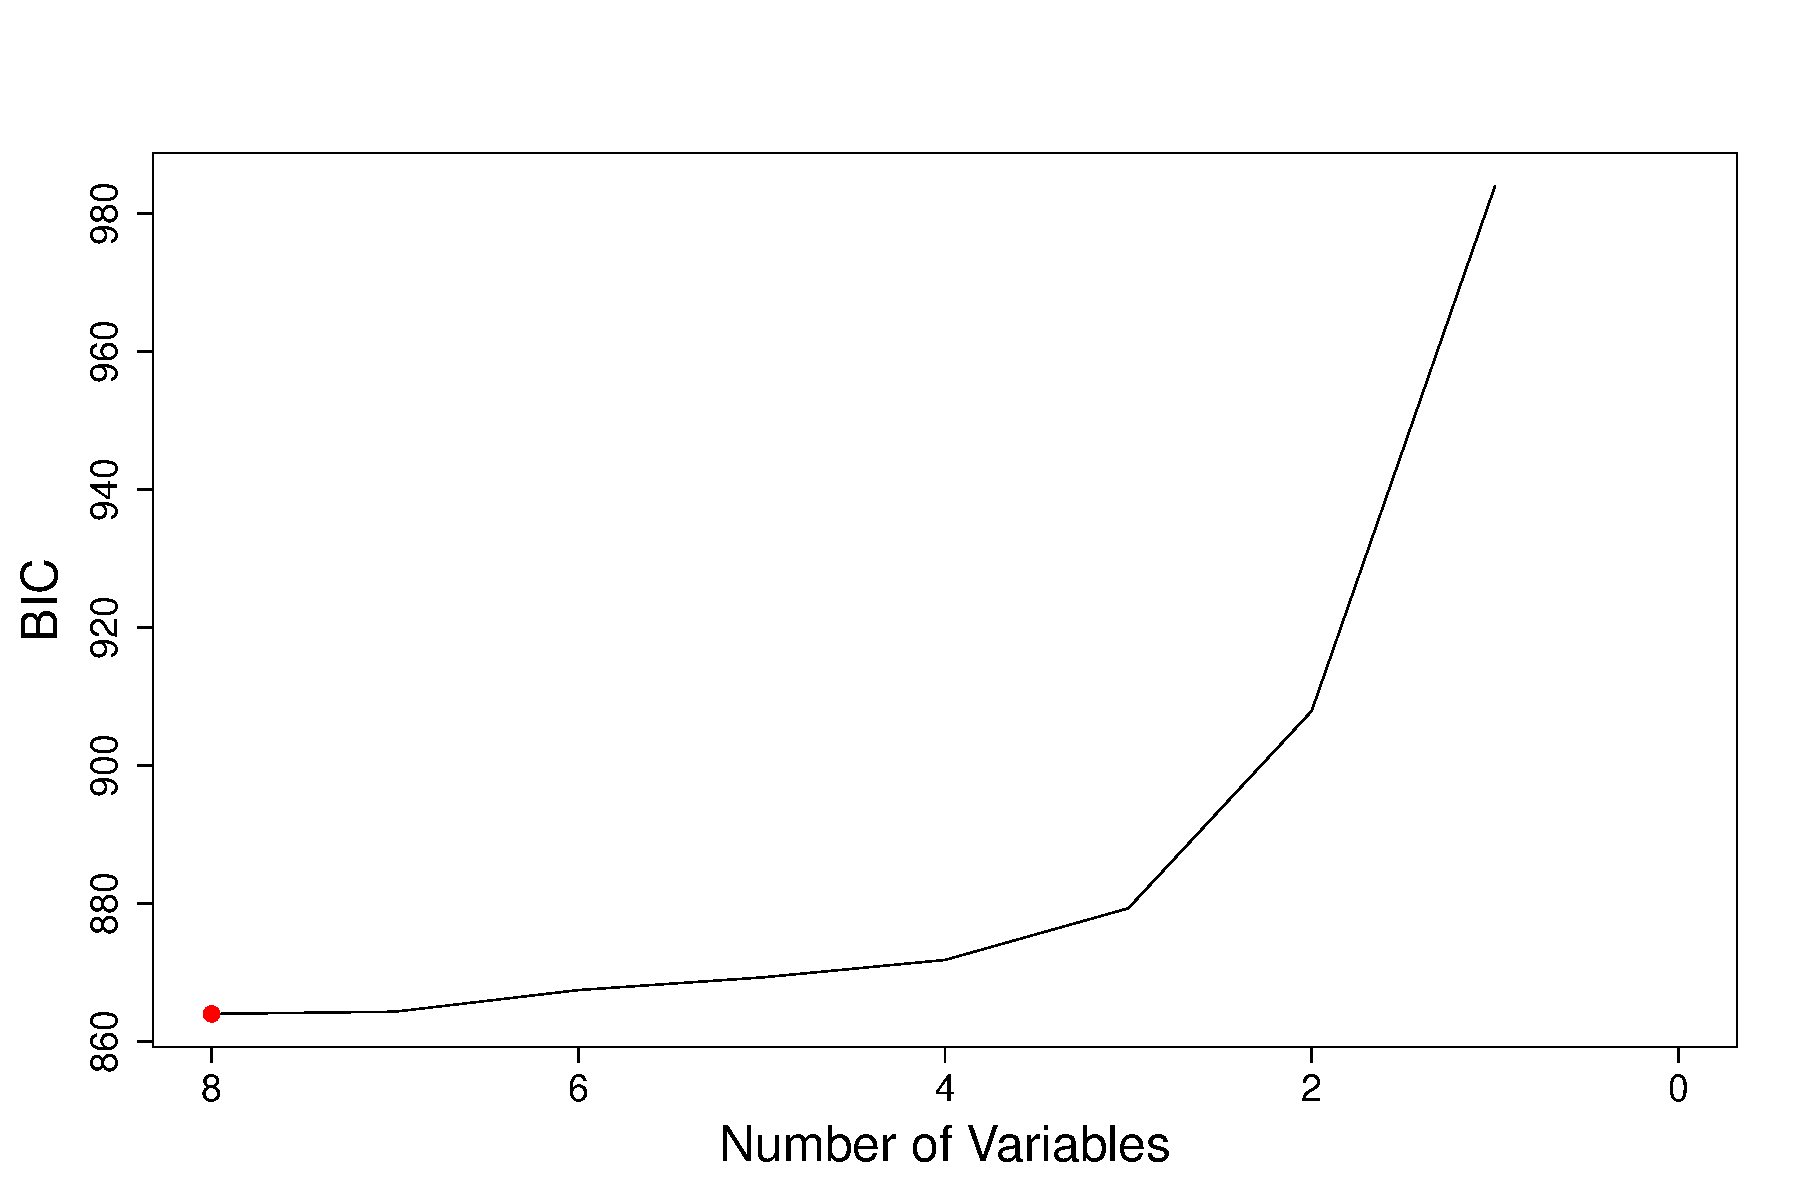
\includegraphics[width=\textwidth]{forward_nvars_workers_binary.pdf}
\caption{Number of variables Forward Selection plots...}
\end{subfigure}
\caption{Workers Binary Variable Selection}
\label{figure:workers_binary_opt}
\end{figure}


\begin{figure}[!tbp]
\begin{subfigure}[b]{0.5\textwidth}
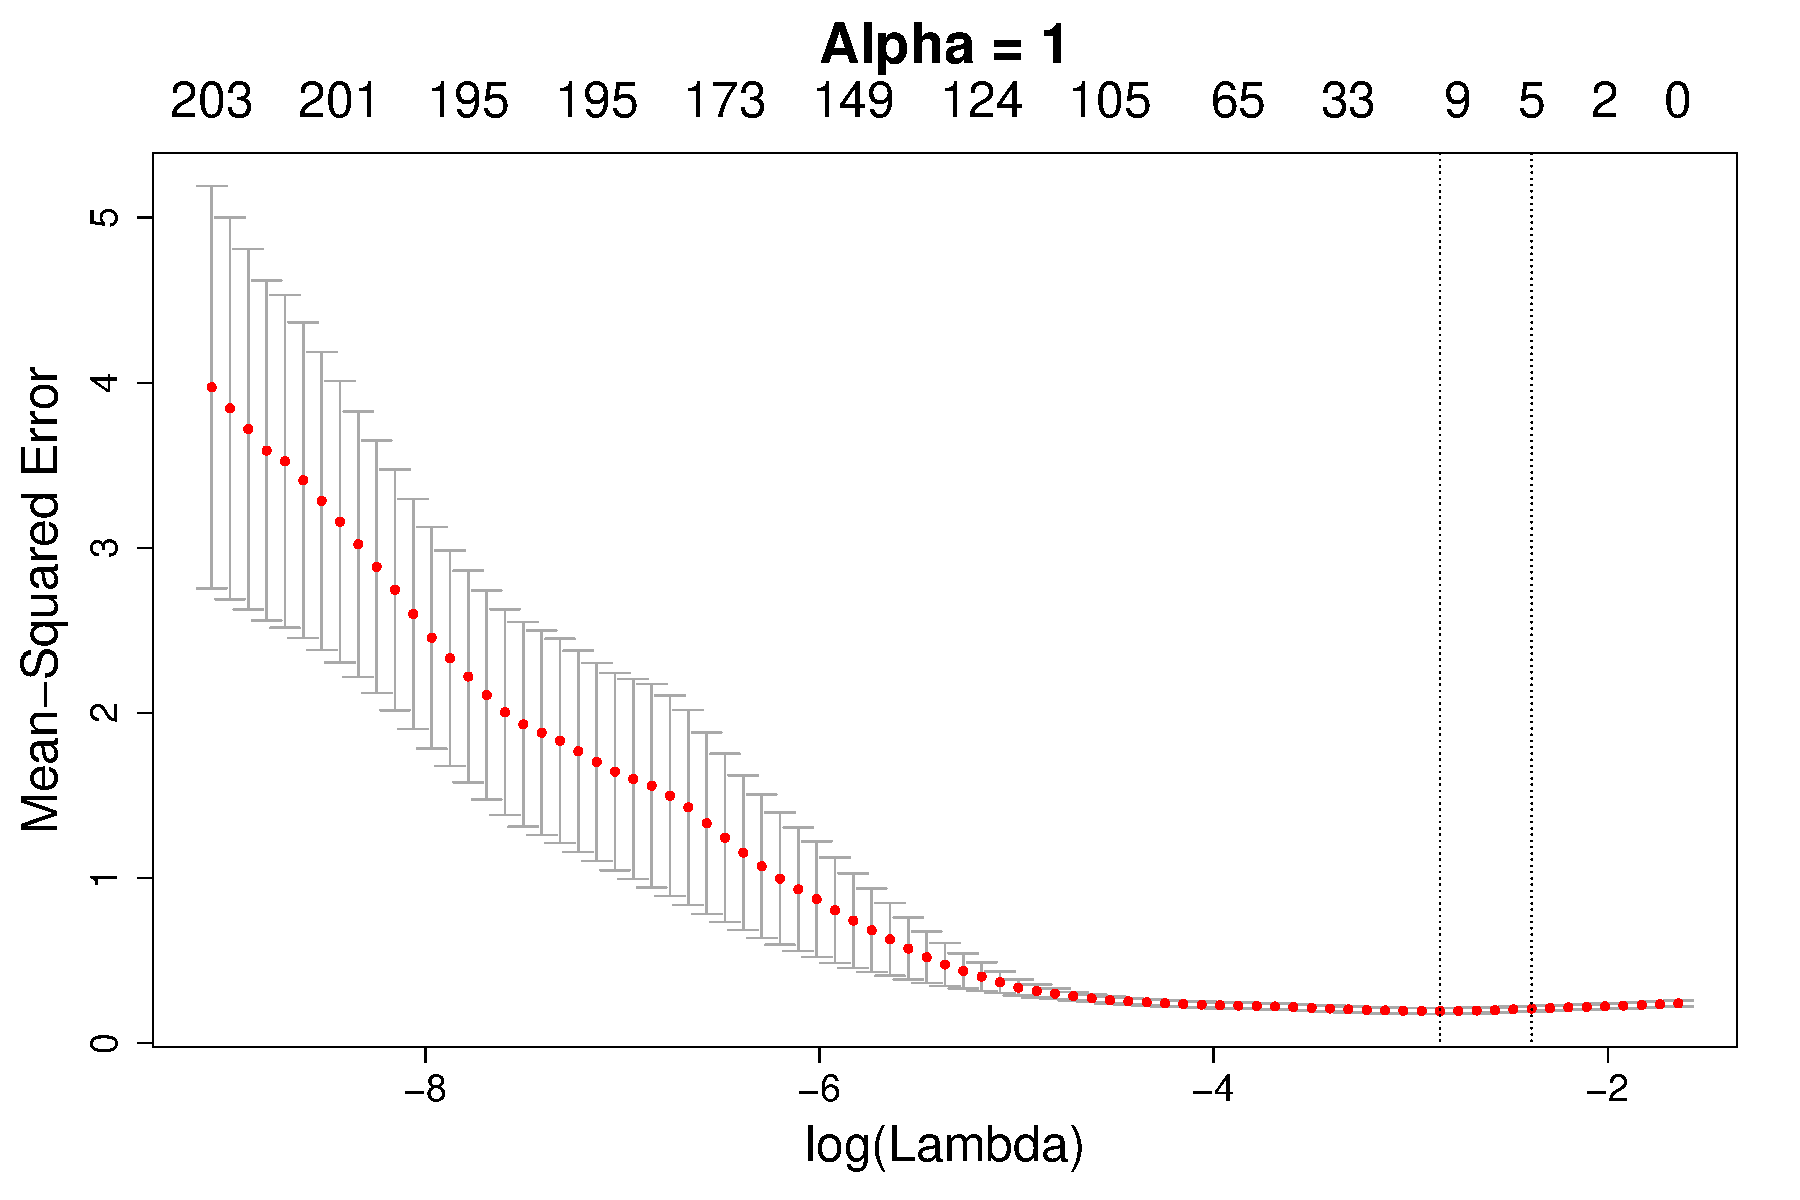
\includegraphics[width=\textwidth]{elastic_cv_workers_nonzero.pdf}
\caption{Cross-validation plots for Elasticnet...}
\end{subfigure}
\hfill
\begin{subfigure}[b]{0.5\textwidth}
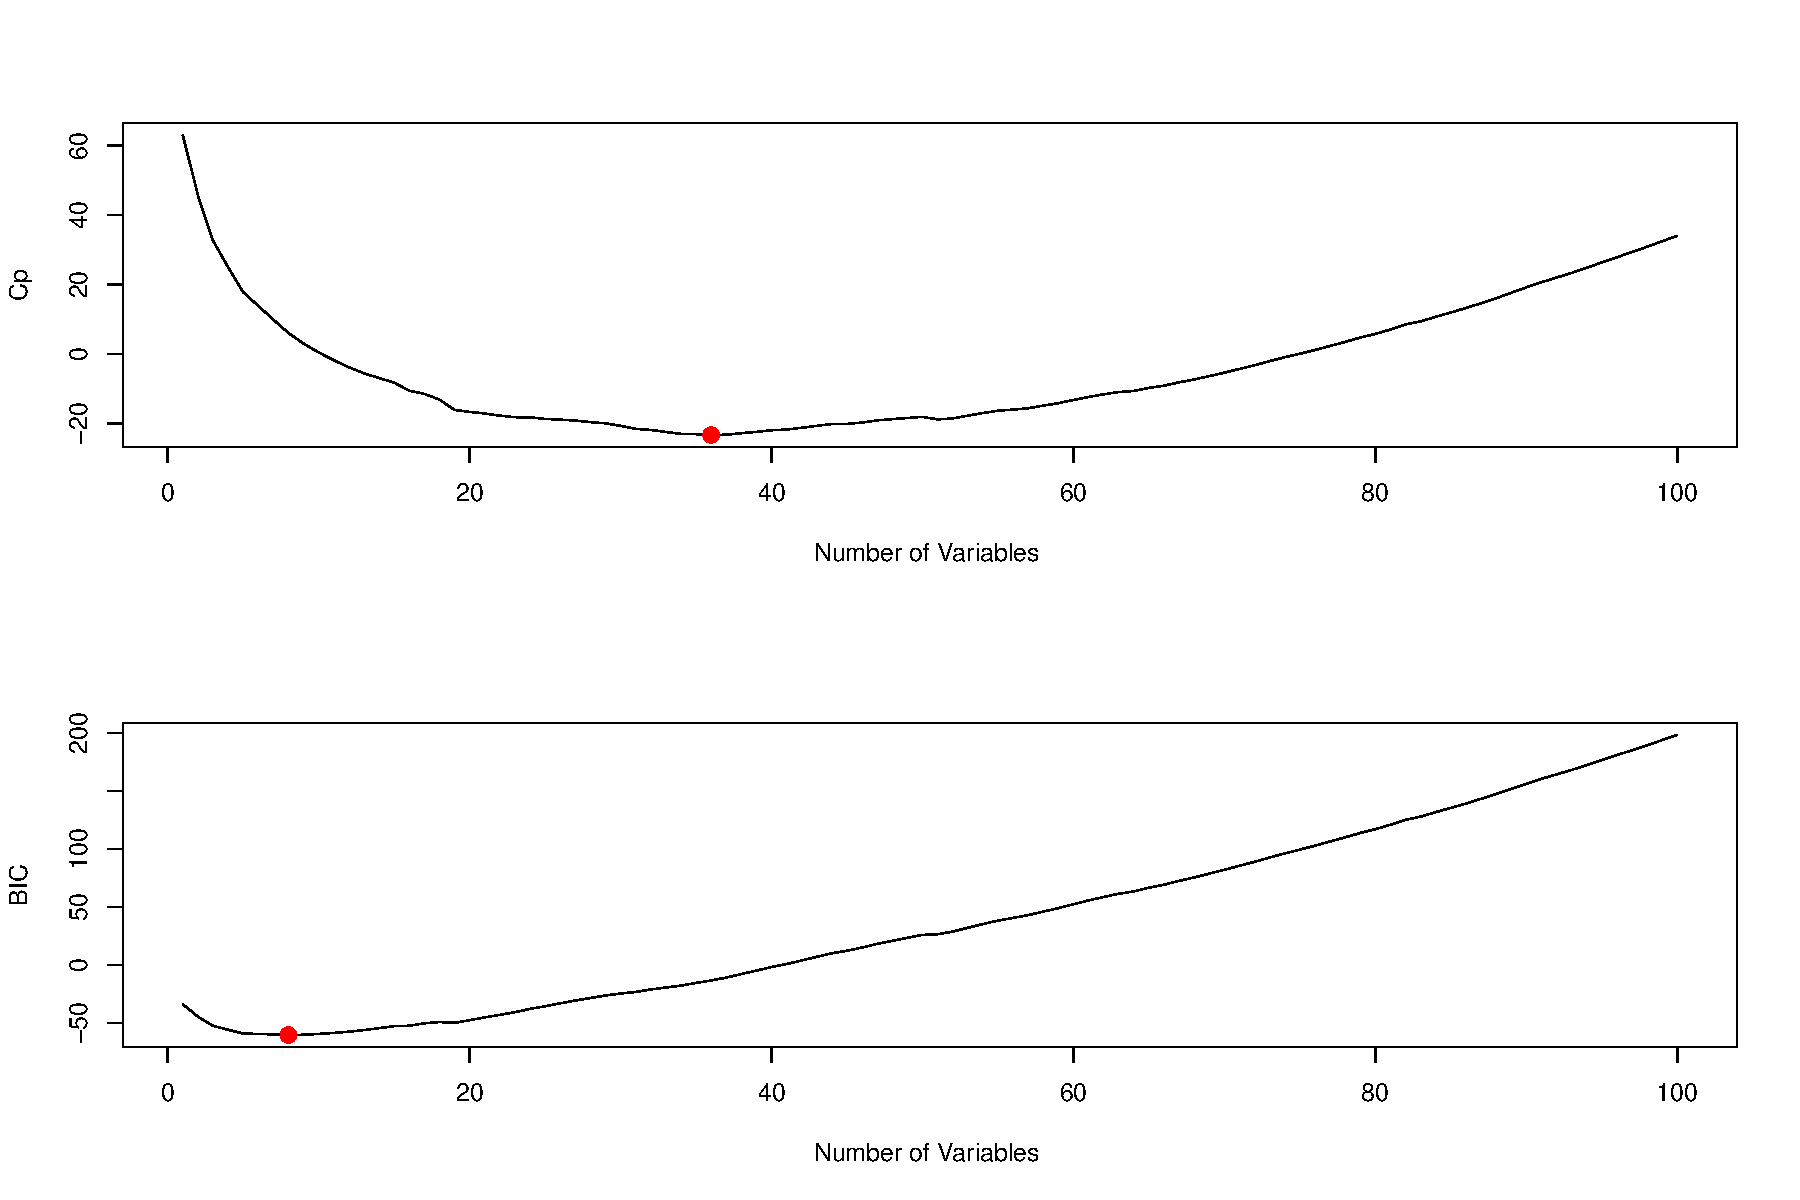
\includegraphics[width=\textwidth]{forward_nvars_workers_nonzero.pdf}
\caption{Number of variables Forward Selection plots...}
\end{subfigure}
\caption{Workers Positive Variable Selection}
\label{figure:workers_nonzero_opt}
\end{figure}

For logistic regression Elasticnet chooses a model of size 6 and Forward Selection chooses a model of size 7. Since these 
models are not much larger the misclassification rates remain at 0.31 and 0.26, respectively. For linear regression, the full 
models for Elasticnet and Forward Selection have a RMSE and $R^2$ of 0.46 and 0.34, respectively. The Elasticnet full model 
has 5 variables and the Forward Selection full model has 8 variables.  In the Appendix, the coefficients estimated for logistic 
regression models can be found in Table \ref{table:workers_binary_full} and the coefficients estimated for linear regression 
models can be found in Table \ref{table:workers_nonzero_full}. 

\subsection{Invasive Species}


\begin{figure}[h]
\centering
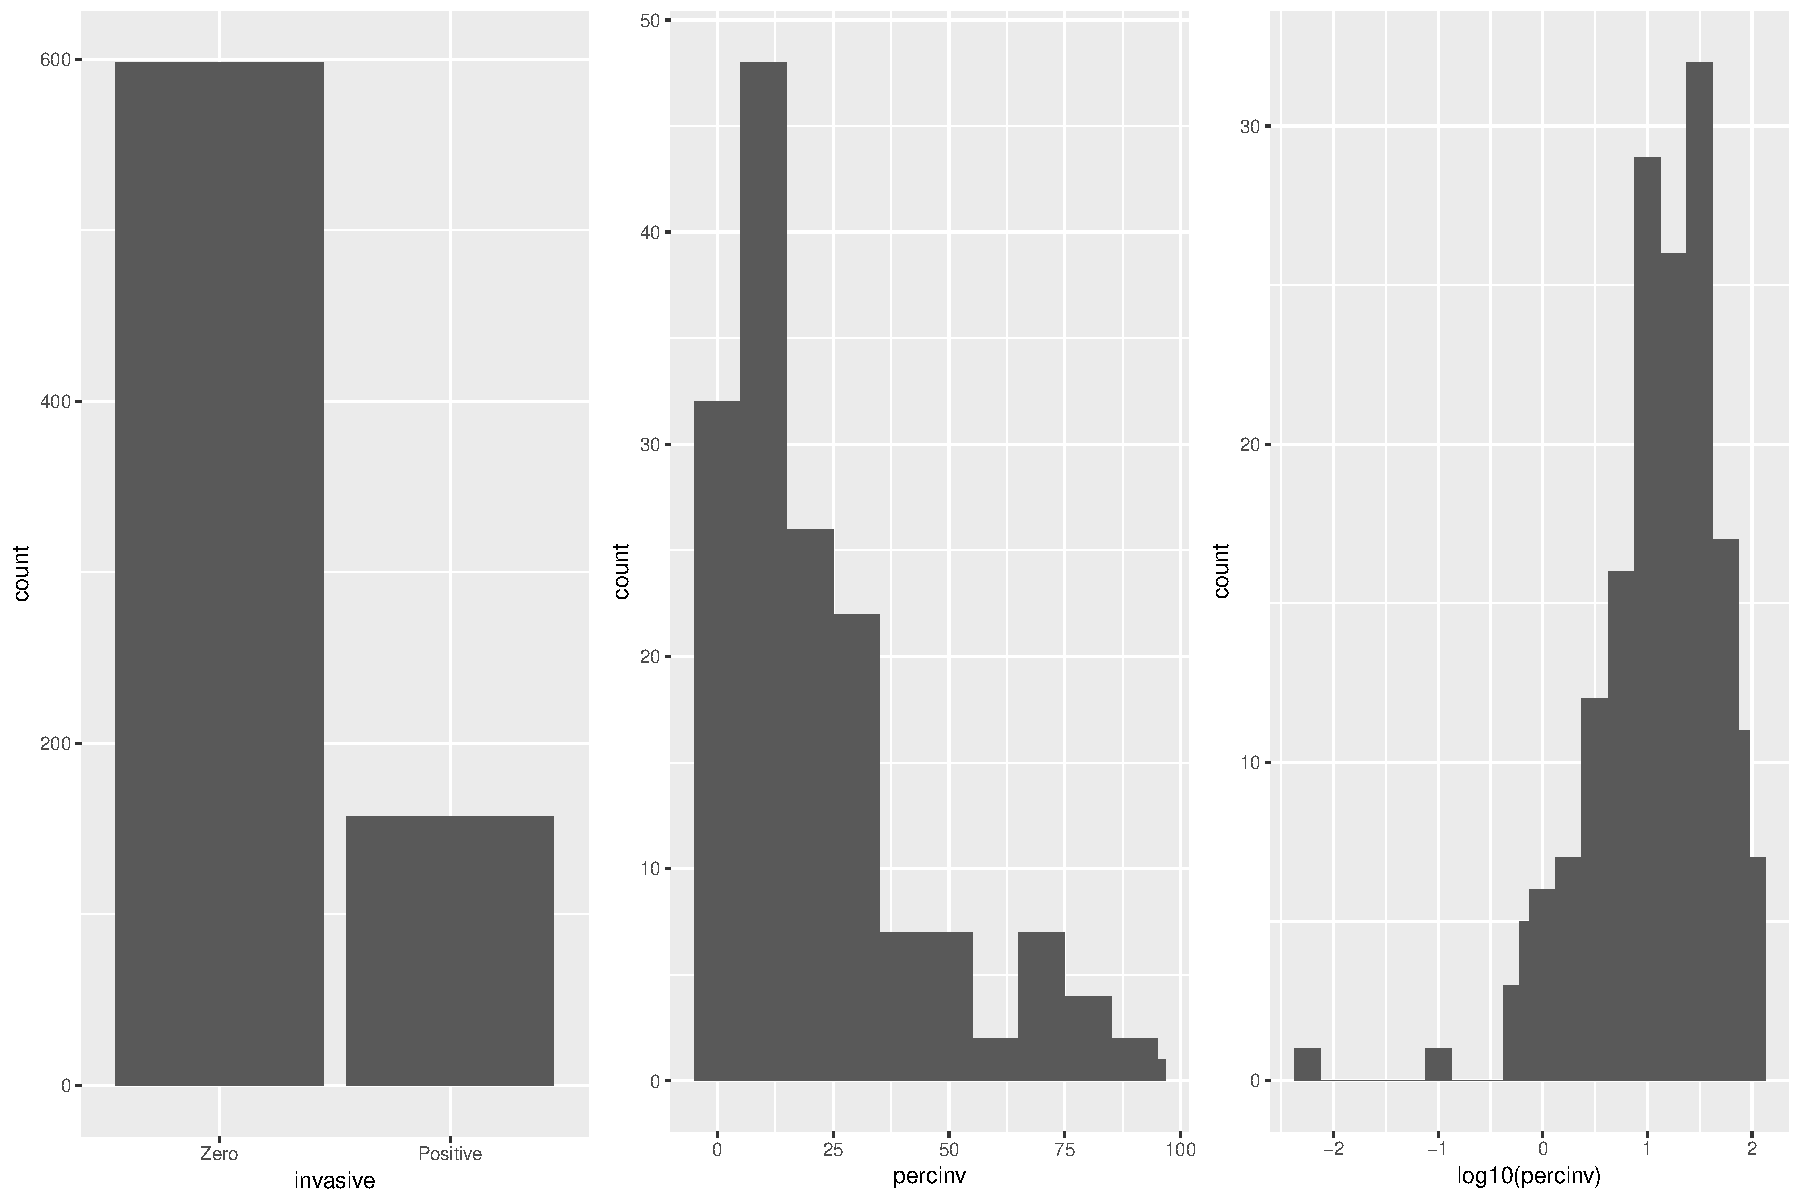
\includegraphics[width = 0.75\textwidth]{invasive_histograms.pdf}
\caption{Histogram of Invasive...}
\label{figure:invasive_hist}
\end{figure}

\begin{table}[h!]
\centering
\begin{tabular}{c|c|c}\hline%
\bfseries \underline{Elasticnet} & \bfseries \underline{Forward~Selection}
\csvreader[head to column names]{invasive_binary_top5names.csv}{}%
{\\\elasticnet & \forward}%
\\\hline
\end{tabular}
\caption{Modeling of Binary Invasive , Top 5 features for each method}
\label{table:invasive_binary_top5}
\end{table}


\begin{figure}[!tbp]
\begin{subfigure}[b]{0.5\textwidth}
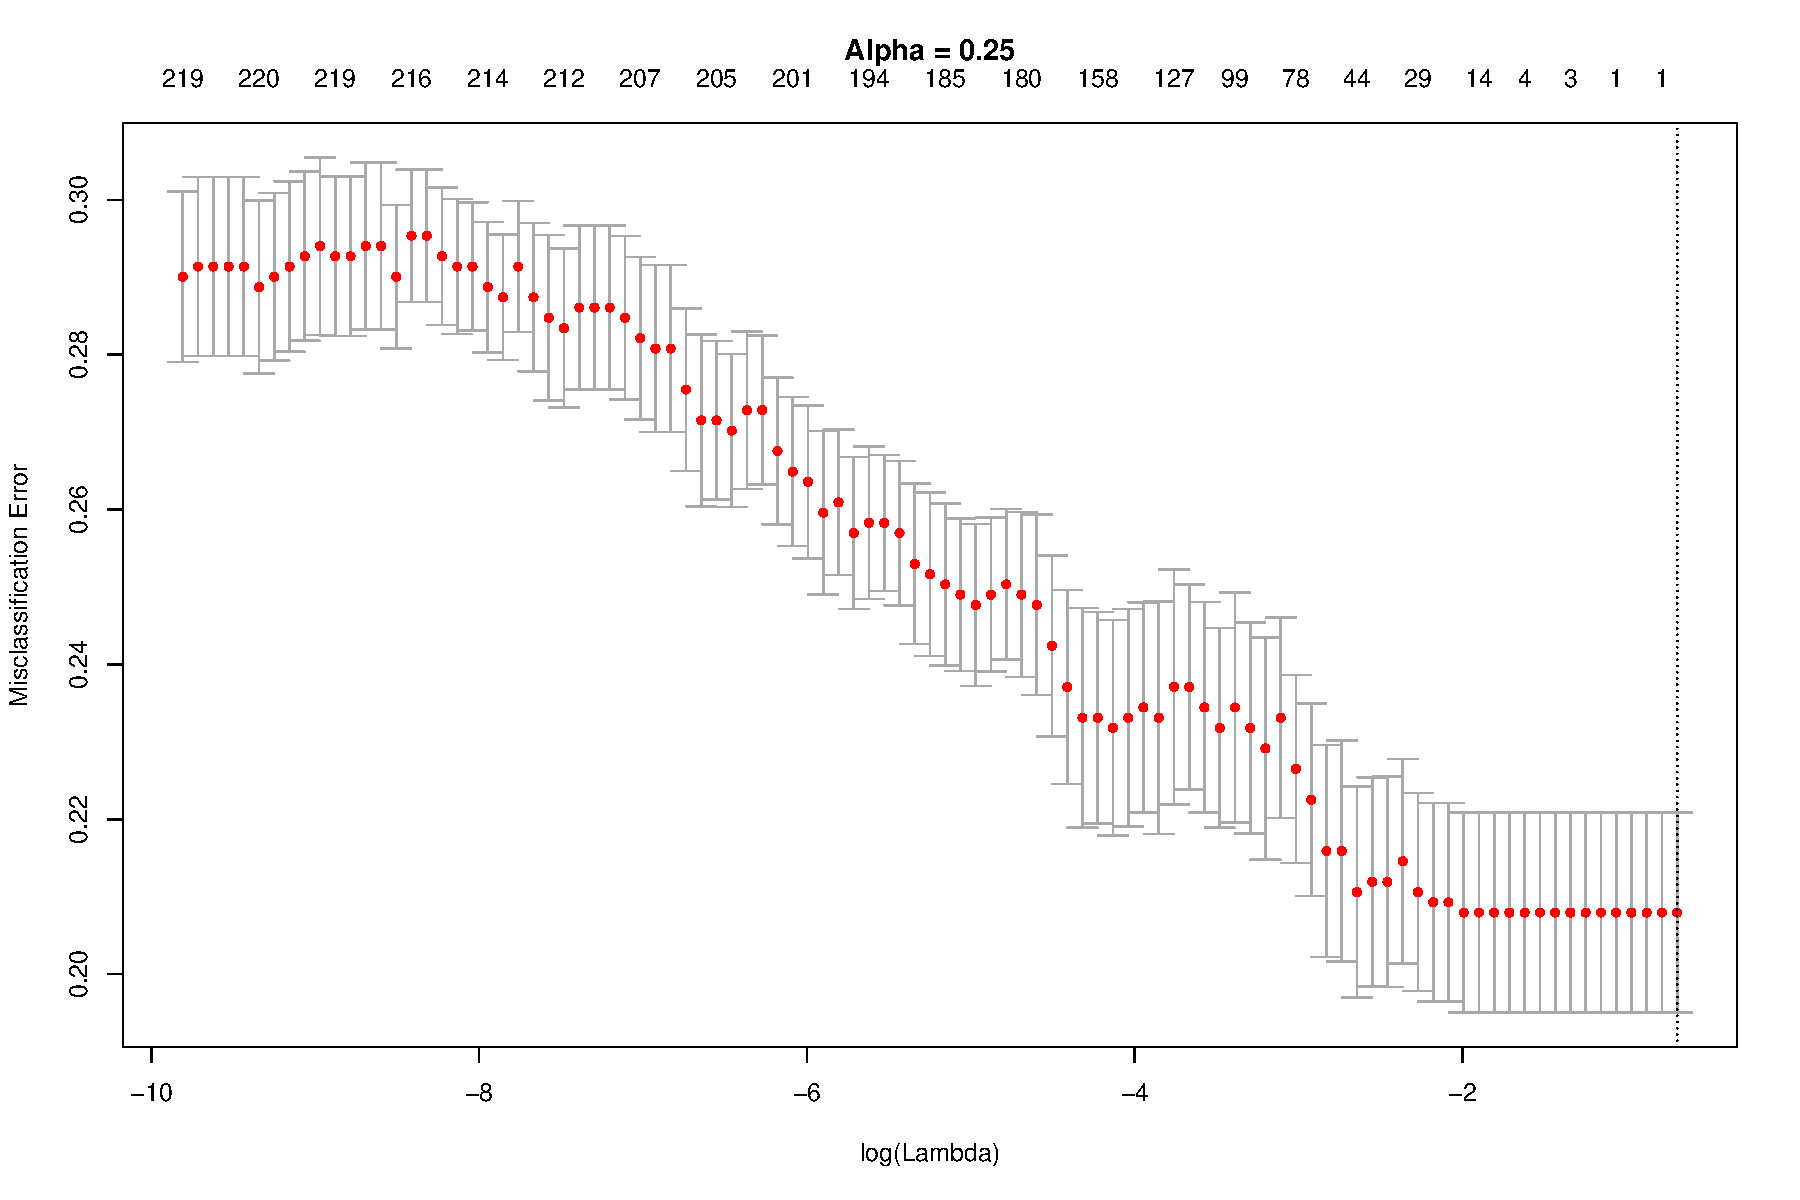
\includegraphics[width=\textwidth]{elastic_cv_invasive_binary.pdf}
\caption{Cross-validation plots for Elasticnet...}
\end{subfigure}
\hfill
\begin{subfigure}[b]{0.5\textwidth}
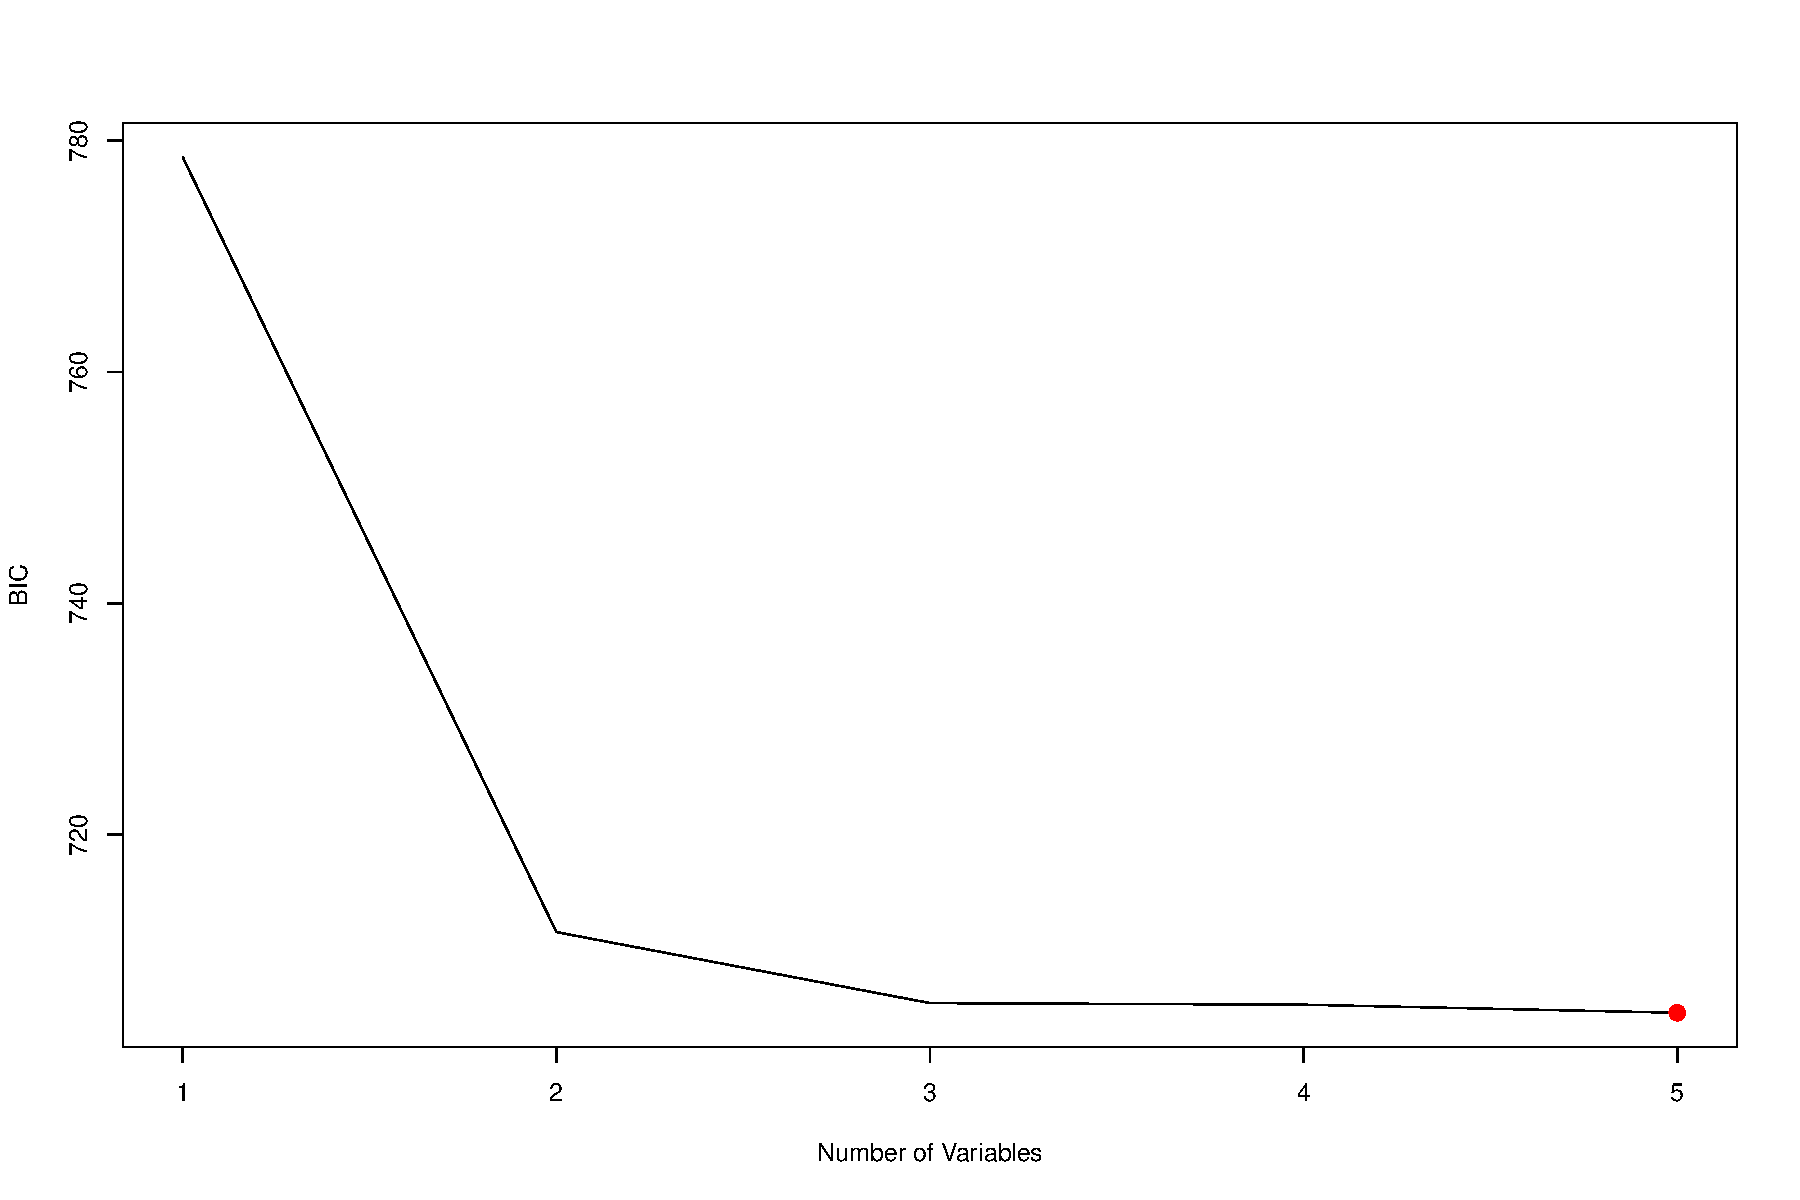
\includegraphics[width=\textwidth]{forward_nvars_invasive_binary.pdf}
\caption{Number of variables Forward Selection plots...}
\end{subfigure}
\caption{Invasive Binary Variable Selection}
\label{figure:invasive_binary_opt}
\end{figure}


\begin{table}[h!]
\centering
\begin{tabular}{c|c|c}\hline%
\bfseries \underline{Elasticnet} & \bfseries \underline{Forward~Selection}
\csvreader[head to column names]{invasive_nonzero_top5names.csv}{}%
{\\\elasticnet & \forward}%
\\\hline
\end{tabular}
\caption{Modeling of Nonzero Invasive , Top 5 features for each method}
\label{table:invasive_nonzero_top5}
\end{table}

\begin{figure}[!tbp]
\begin{subfigure}[b]{0.5\textwidth}
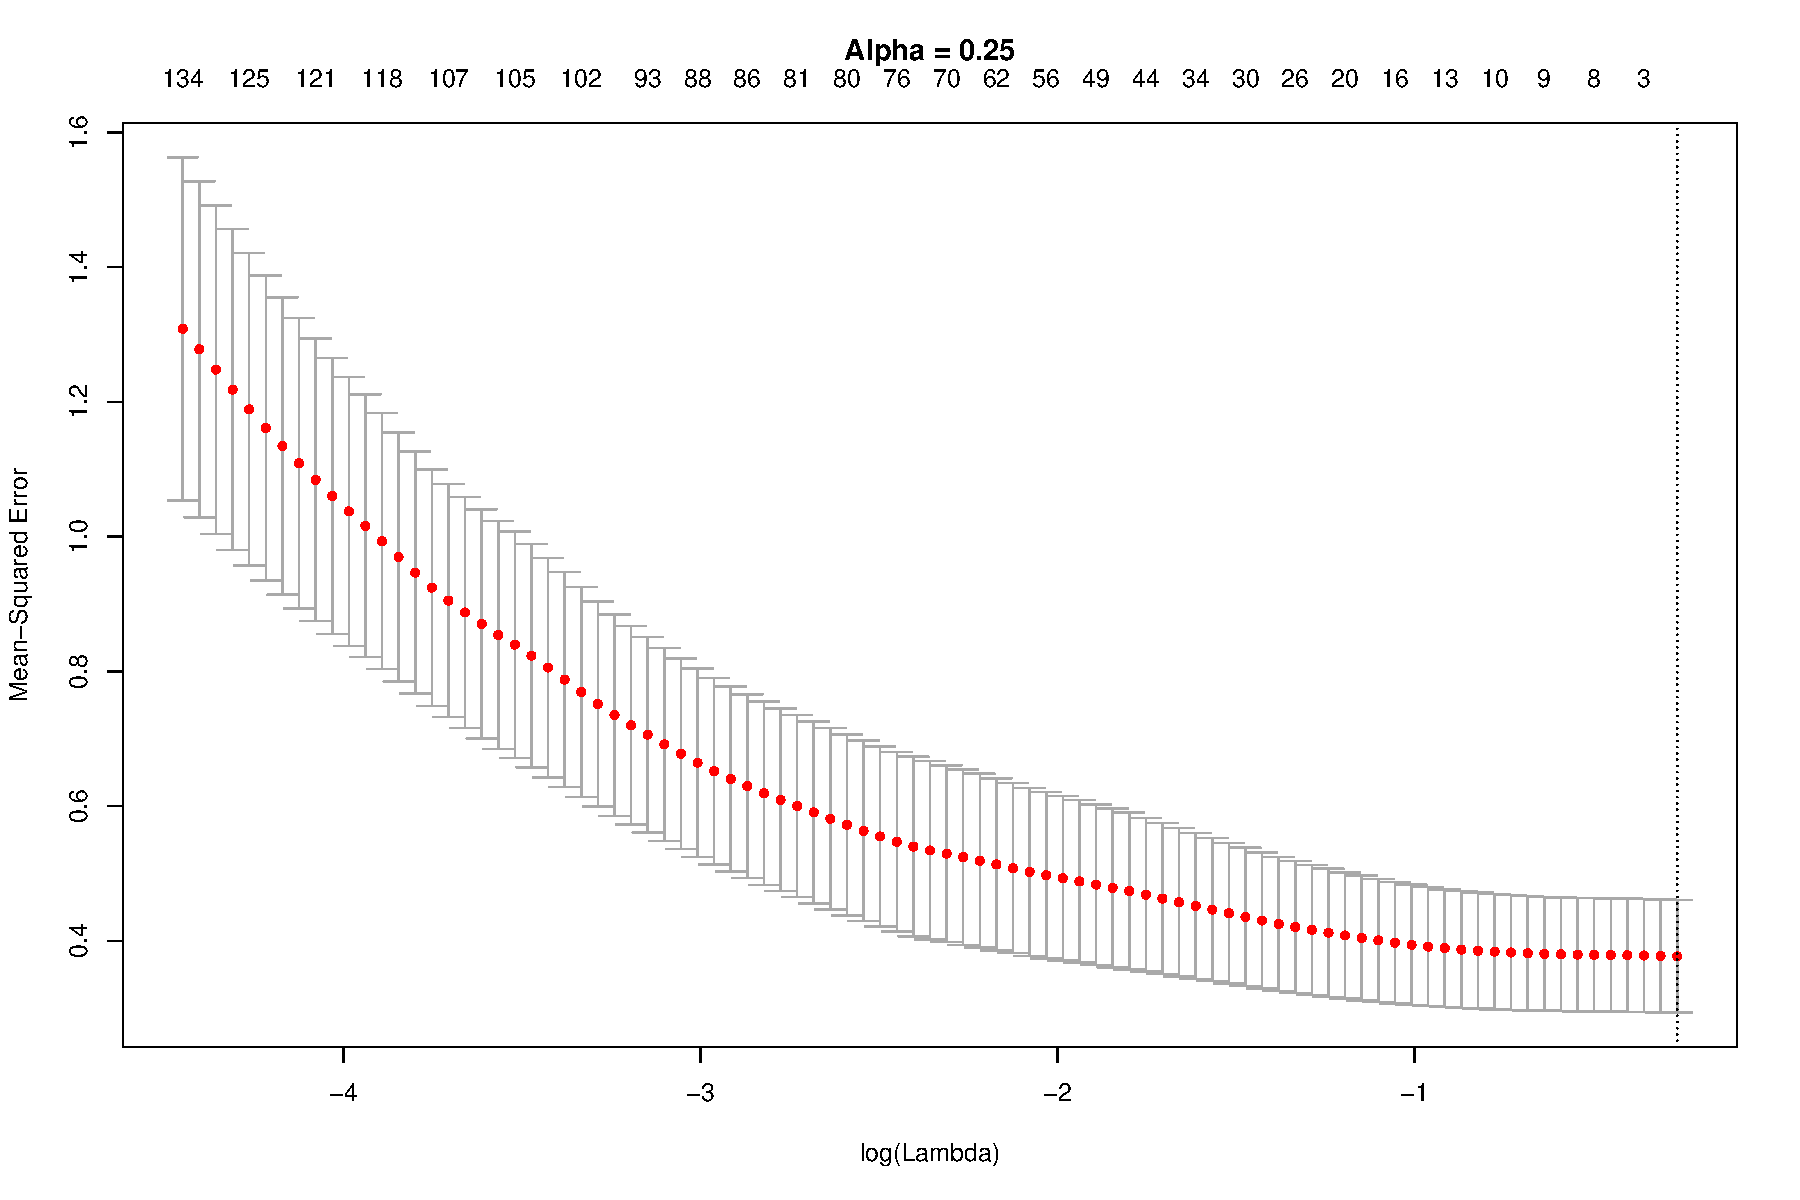
\includegraphics[width=\textwidth]{elastic_cv_invasive_nonzero.pdf}
\caption{Cross-validation plots for Elasticnet...}
\end{subfigure}
\hfill
\begin{subfigure}[b]{0.5\textwidth}
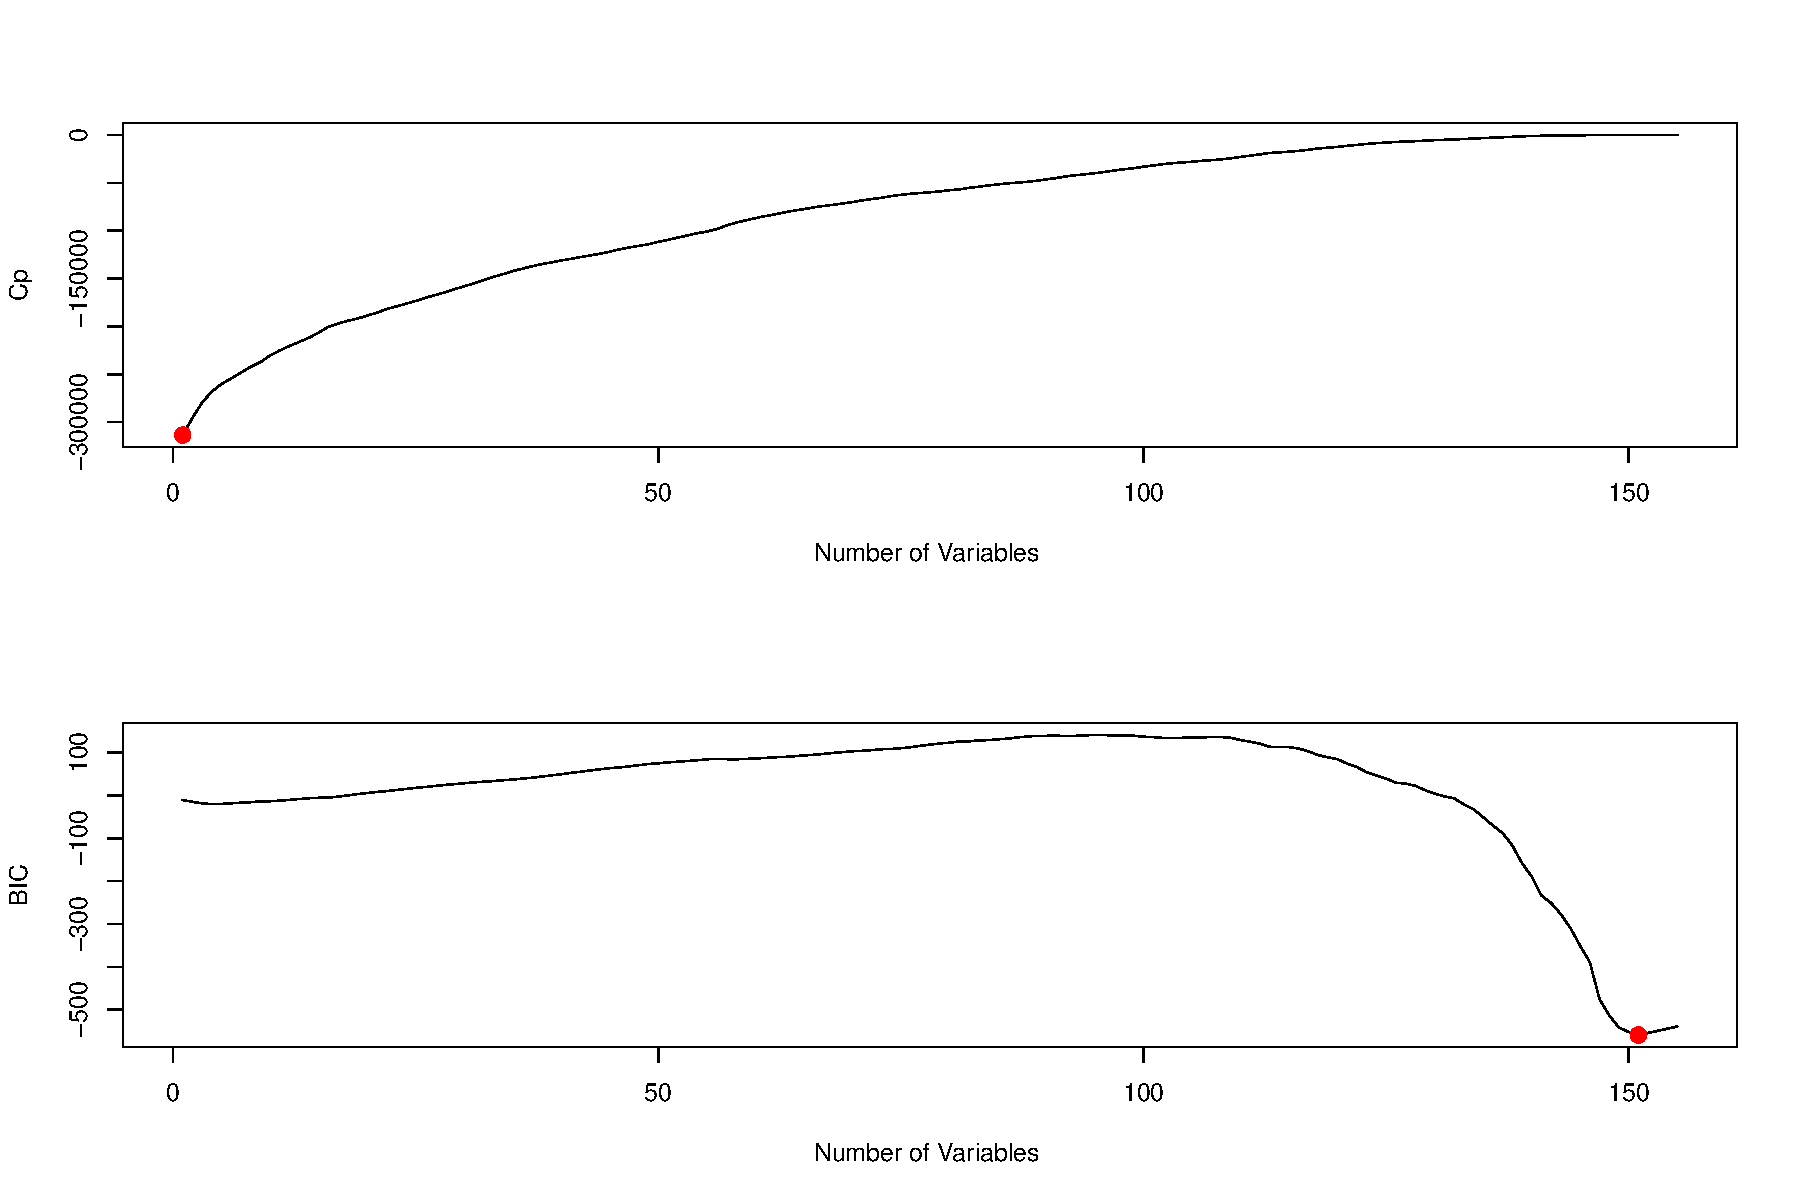
\includegraphics[width=\textwidth]{forward_nvars_invasive_nonzero.pdf}
\caption{Number of variables Forward Selection plots...}
\end{subfigure}
\caption{Invasive Positive Variable Selection}
\label{figure:invasive_nonzero_opt}
\end{figure}


\subsection{Land use choices}


\section{Statistical Methods} \label{stat_methods}

\subsection{Generalized Linear Models}

\[\bY = \bX\beta + \epsilon \tag{1}\]
%\[Y_i =  \sum_{j=1}^{p} X_{i,j}\beta_j + \epsilon \tag{1}\]

Standard Linear Regression can be represented in matrix form as seen in equation 1 above, When there are $n$ observations and $p$ predictor variables,  $\bY$ is a $n \times 1$ vector of the outcome variable, $\bX$ is a $n \times p$ matrix of predictor variables, $\bbeta$ is a $p \times 1$ vector of variable coefficients and $\epsilon$ is the error 
term. The standard linear model works best when the outcome variable $\bY$ has a normal distribution, and therefore takes 
continuous values. When the outcome variable is continuous, but not normal shaped (e.g., skewed like the productivity 
data) it can be possible to transform the data by taking the logarithm or something similar. However, when the outcome 
variable is discrete (such as binary labels of 1 and 0 denoting absence/presence of a feature) a further modification must be made. The outcome variable is clearly no longer normally distributed, as it is not even continuous. Without modification we could get predicted values below 0, above 1 or somewhere in between, none of which make much sense.

This calls for the use of logistic regression, in which we perform a logit transformation as seen in the equation below so that the 
$\bX\beta$ can still be mapped to a continuous scale. In some respects this is a computational concern, but it also changes the 
way coefficients can be interpreted. For example, instead of a one unit change in $X_1$ predicting a $\beta_1$ change in the predicted $Y$, 
in this case it predicts a $\beta_1$ change in the log odds of $Y$.

\[log \frac{\Pr(Y = 1)}{\Pr(Y = 0)} = \bX\beta \]

This equation can be rewritten as below

\[ \Pr(Y = 1) = \frac{e^{\bX\beta}}{1 + e^{\bX\beta}} \]

Multiclass Logistic Regression

\[ \Pr(Y = k) = \frac{e^{\bX\beta_k}}{\sum_{l=1}^{K-1} e^{\bX\beta_l}} \]

% include Poisson function

\subsection{Performance Measures}

There are many measures of fit for linear models. When there are many possible predictor variables, care must be taken 
to use appropriate measures, as some measures will favor just adding all of the variables to the model. For example, if we 
aim to minimize the mean square error adding more predictor variables to the model will always be encouraged. Since that is 
not desired, measurements like Bayesian Information Criterion (BIC) can be used. BIC is a combination of how well the model 
fits the data and a penalty term for the number of predictor variables included in the model. The goal is to minimize BIC, that is 
the model with the best balance of small size and goodness of fit. BIC is chosen over other potential measurements because it 
puts a large penalty on the inclusion of additional variables.

Another approach is to use cross-validation. In this technique the dataset is first split into $k$ equally sized sets. Then a 
model is fit using $k - 1$ of the sets (training sets) and evaluated on the remaining 1 (test) set. This is repeated $k$ times, 
each time reserving a different 1 test set, and then results across the $k$ runs are averaged. The benefit of this is that model 
building and model evaluating are happening on different portions of the data, so we can distinguish if the model is picking up 
on generalizable patterns or just random noise. Using cross-validation the average test set mean square error is an 
appropriate measure of model fit. We can also capture the standard deviation across the $k$ runs to measure variability, which is shown in the error bars of the Elasticnet cross-validation plots.

\subsection{Best Subset and Forward Selection}

The essential goal of variable selection is to find the best combination of predictor variables to explain the outcome variable. As 
discussed above, when we have many possible predictors we often want to put a constraint on the problem so that all variables 
are not included. Such a constraint might be limiting the number of variables included or that the model found can generalize to 
other data. Best subset selection, the most natural, but computationally difficult way is to try all possible combinations of 
variables and select the best fitting combination. However, when the number of variables, $p$, is large this quickly becomes 
infeasible, as there are $2^p$ possible combinations. 

One approach to tackle the computational complexity discussed above is to restrict the search for the optimal number of 
predictor variables, which is what Forward Selection does. In this algorithm, we start with an empty model and iteratively add a 
new variable at each stage that most increases the fit. This procedure can work well, but may not find the optimal solution. As 
an example, consider a case where $X_1$ is the single most predictive variable, but the combination of $X_2$ and $X_3$ is 
the best two variable combination. The algorithm will first add $X_1$, but then regardless whether it adds $X_2$ or $X_3$ next, 
it will have found a suboptimal solution. In general, we can decide to stop adding variables once we have reached an optimal 
performance measure like BIC or cross-validation test error.


\subsection{Regularized Regression}

	\[\min_{\beta}  \|\bY - \bX\beta\|_{2}^{2} \tag{linear model}\]
	\[\min_{\beta}  \|\bY - \bX\beta\|_{2}^{2} + \lambda||\beta||_2^2 \tag{ridge regression}\]
	\[\min_{\beta}  \|\bY - \bX\beta\|_{2}^{2} + \lambda||\beta|| \tag{LASSO}\]

The above notation of $||\cdot||_{2}^{2}$ and  $||\cdot||$ are defined in general as: $||\bX||_{2}^{2} = x_1^2 + x_2^2 + ... + 
x_n^2$ and $||\bX|| = |x_1| + |x_2| + ... + |x_n|$. As shown in equation ? in the standard linear model, we try to find the $\beta$, that is a vector of coefficients,  
that minimizes the squared difference between the true $\bY$ and the predicted $\hat{\bY}$ (which is $\beta\bX$). In 
regularized regression we do the same thing, but also add a second term that we look to simultaneously minimize. This second 
term adds a penalty for increasing values of $\beta$, so the two terms must be balanced. The optimal model will find a balance 
between fitting the outcome variable closely, but not having too large of coefficient values. The difference between Ridge 
regression and LASSO is how we add up the coefficients. In Ridge Regression the coefficients are squared and then summed, 
in LASSO we take the absolute value of 
the coefficients and then sum them. LASSO will encourage most of the coefficients to go to zero, thus only including a small 
number of terms in the model. Ridge regression will encourage the coefficient values to be spread out among predictor 
variables, leaving all of the variables in the model, but helping to offset negative effects of correlated predictor variables. 

\[\min_{\beta}  \|\bY - \bX\beta\|_{2}^{2} + \lambda[(1 - \alpha)||\beta||_2^2 + \alpha||\beta||] \tag{ElasticNet}\]

The technique that is used in this analysis is a combination of the Ridge and LASSO penalties, called ElasticNet. As can be seen in the equation above both the square of the coefficients and the absolute value of the coefficients is included, with the contribution of each controlled by the size of $\alpha$ which takes a value between 0 and 1. ElasticNet, thus combines the favorable properties of Ridge and LASSO, in that it can achieve both sparse models and can handle correlated predictor variables. Both the $\lambda$ and the $\alpha$ can be set using cross-validation (as discussed above) to be appropriate values for the particular dataset. 

\section{Limitations and Future Work}
There are a few key considerations that should be kept in mind when interpreting this analysis. First, is that relationships discovered in this analysis are correlational nature and cannot be assumed to be causal. Just because farms with a higher coverage of invasive species have lower productivity does not necessarily mean the invasive species causes lower productivity. It could be that lower productivity causes higher invasive species coverage. Or there could other factors not captured in the model that influence both productivity and invasive species. In order to determine causality, relationships of interest should be tested in a designed experiment. 

Secondly, p-values and confidence intervals for coefficients were intentionally not included in the analysis. In standard 
regression analysis we pre-specify the model and then test which variables are found to be significant. However, when using 
Elasticnet and Forward Selection like we have done here, we do not specify the model ahead of time, but instead let the data 
decide the model. This violates the significance test assumption and can lead to misleadingly small p-values. While there are some advanced techniques to try to adjust for this, it is recommended to view the results in this report as an exploratory analysis rather than definitive evidence.

Future analysis might look to explore better fitting relationships, particularly for the outcome variables that had poor RMSE and $R^2$ values. The relationships modeled in this report only considered linear combinations of predictor variables to predict/explain the outcome variables. Modifications could include adding interaction terms (i.e., $x_1x_2$) or nonlinear terms (i.e., $x_1^2$ or binary transformations $x_1 > 10$). Exploring all possible modifications of this type is not computationally feasible, but with domain knowledge a subset of theorized relationships could be tested. Lastly, the variables used here primarily covered socioeconomic dimensions. The addition of physical and biotic variables may help better predict/explain the outcome variables or may change the importance of previously highlighted socioeconomic variables.


\medskip

\small

\begin{thebibliography}{99}




\end{thebibliography}

\section{Appendix}

\begin{table}[h!]
\begin{tabular}{l|c|c}\hline%
\bfseries \underline{Variable} & \bfseries \underline{Elasticnet} & \bfseries \underline{Forward~Selection}
\csvreader[head to column names]{fullcoeflist_production.csv}{}%
{\\\variable & \elastic & \forward}%
\\\hline
\end{tabular}
\caption{Full coefficient list for Production model}
\label{table:prod_full}
\end{table}

\begin{figure}[h]
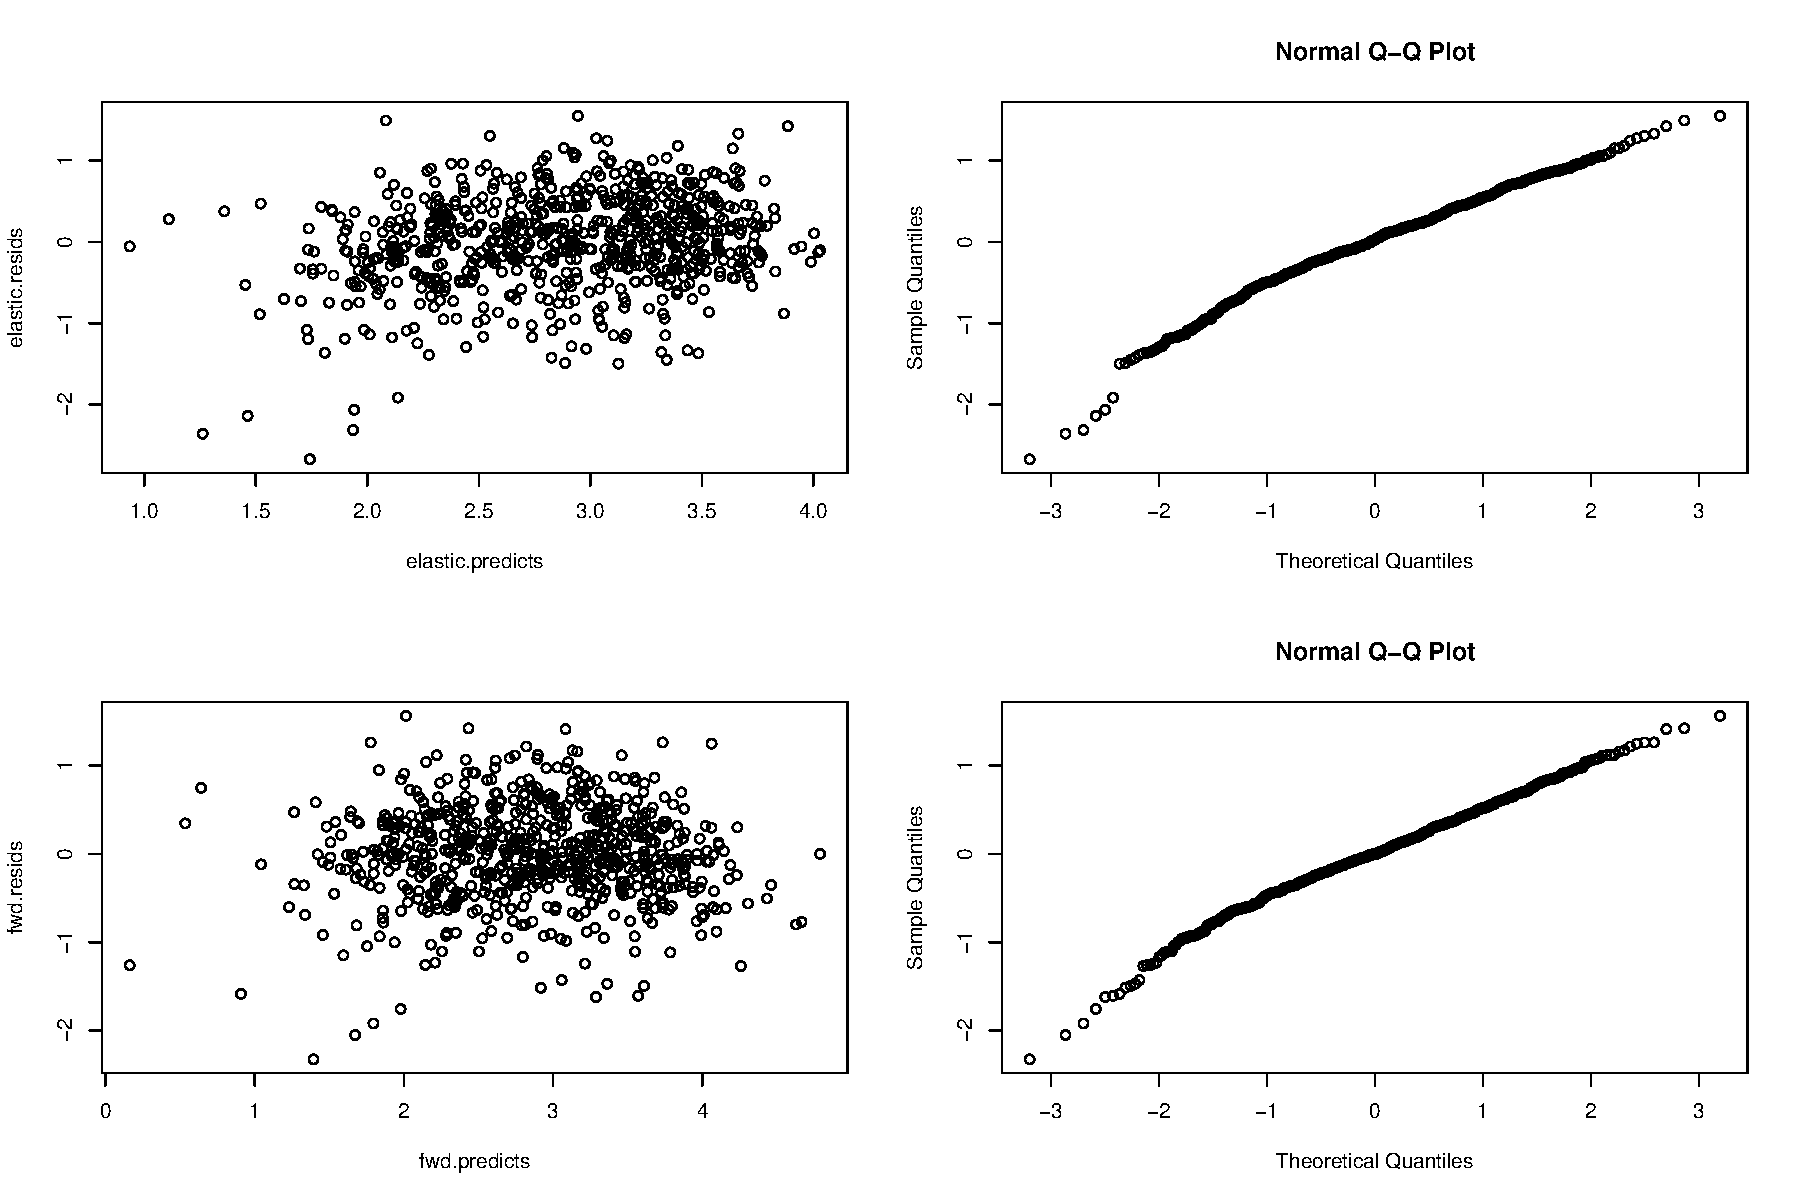
\includegraphics[width = \textwidth]{resids_production.pdf}
\caption{Diagnostic Residual plots for Production. The plots on the left show the predicted values vs. the residuals and both demonstrate a desirable lack of pattern. The plots of the right examine the normality of the residuals, both staying close to the desired straight diagonal pattern. }
\label{figure:resids_prod}
\end{figure}


\begin{table}[h!]
\begin{tabular}{l|c|c}\hline%
\bfseries \underline{Variable} & \bfseries \underline{Elasticnet} & \bfseries \underline{Forward~Selection}
\csvreader[head to column names]{fullcoeflist_netincome.csv}{}%
{\\\variable & \elastic & \forward}%
\\\hline
\end{tabular}
\caption{Full coefficient list for Net Income model}
\label{table:netincome_full}
\end{table}

\begin{figure}[h]
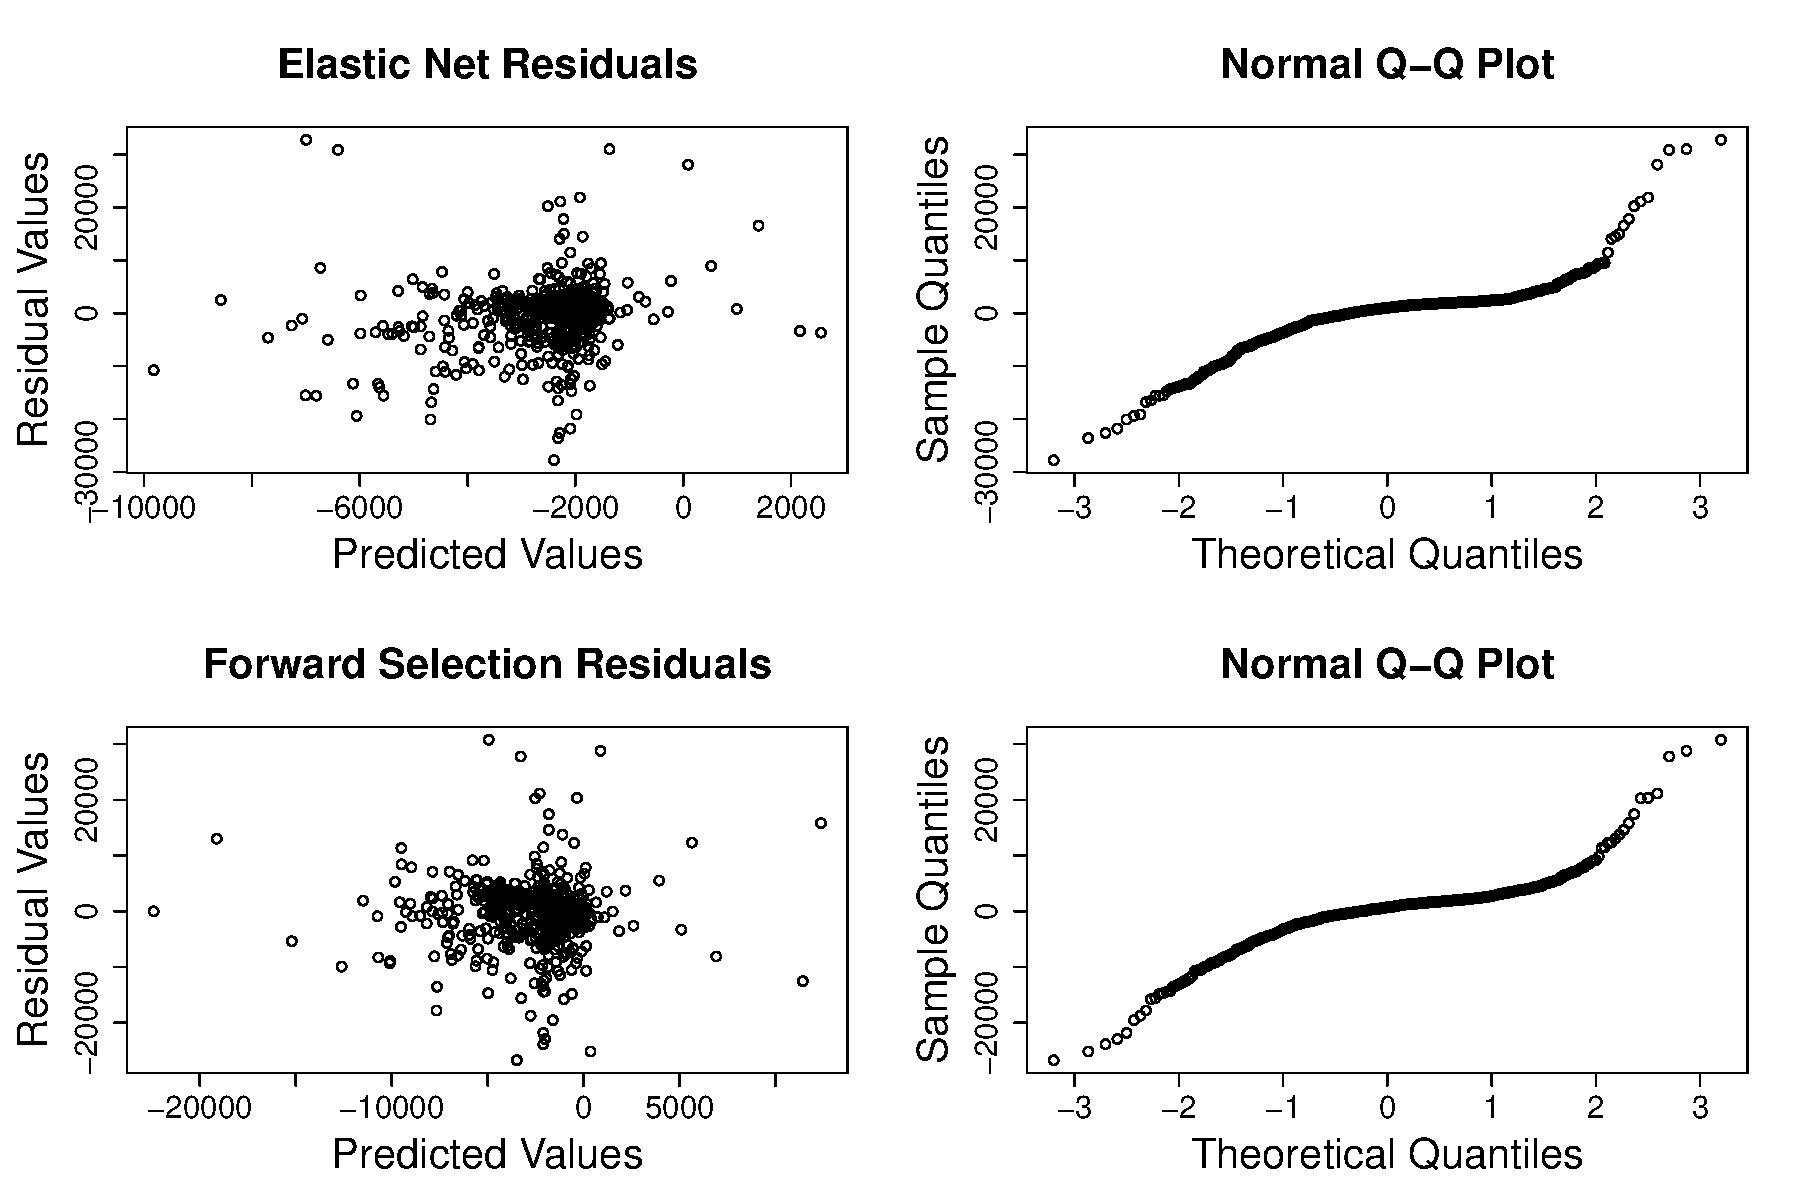
\includegraphics[width = \textwidth]{resids_netincome.pdf}
\caption{Diagnostic Residual plots for Net Income. The plots of the predicted values vs. the residuals both demonstrate a desirable lack of pattern. The plots examining the normality of the residuals do not follow a diagonal line as closely as would be hoped, but not an extreme departure.}
\label{figure:resids_netincome}
\end{figure}

\begin{table}[h!]
\begin{tabular}{l|c|c}\hline%
\bfseries \underline{Variable} & \bfseries \underline{Elasticnet} & \bfseries \underline{Forward~Selection}
\csvreader[head to column names]{fullcoeflist_workers_binary.csv}{}%
{\\\variable & \elastic & \forward}%
\\\hline
\end{tabular}
\caption{Full coefficient list for Binary Workers model}
\label{table:workers_binary_full}
\end{table}

\begin{table}[h!]
\begin{tabular}{l|c|c}\hline%
\bfseries \underline{Variable} & \bfseries \underline{Elasticnet} & \bfseries \underline{Forward~Selection}
\csvreader[head to column names]{fullcoeflist_workers_nonzero.csv}{}%
{\\\variable & \elastic & \forward}%
\\\hline
\end{tabular}
\caption{Full coefficient list for Nonzero Workers model}
\label{table:workers_nonzero_full}
\end{table}

\begin{figure}[h]
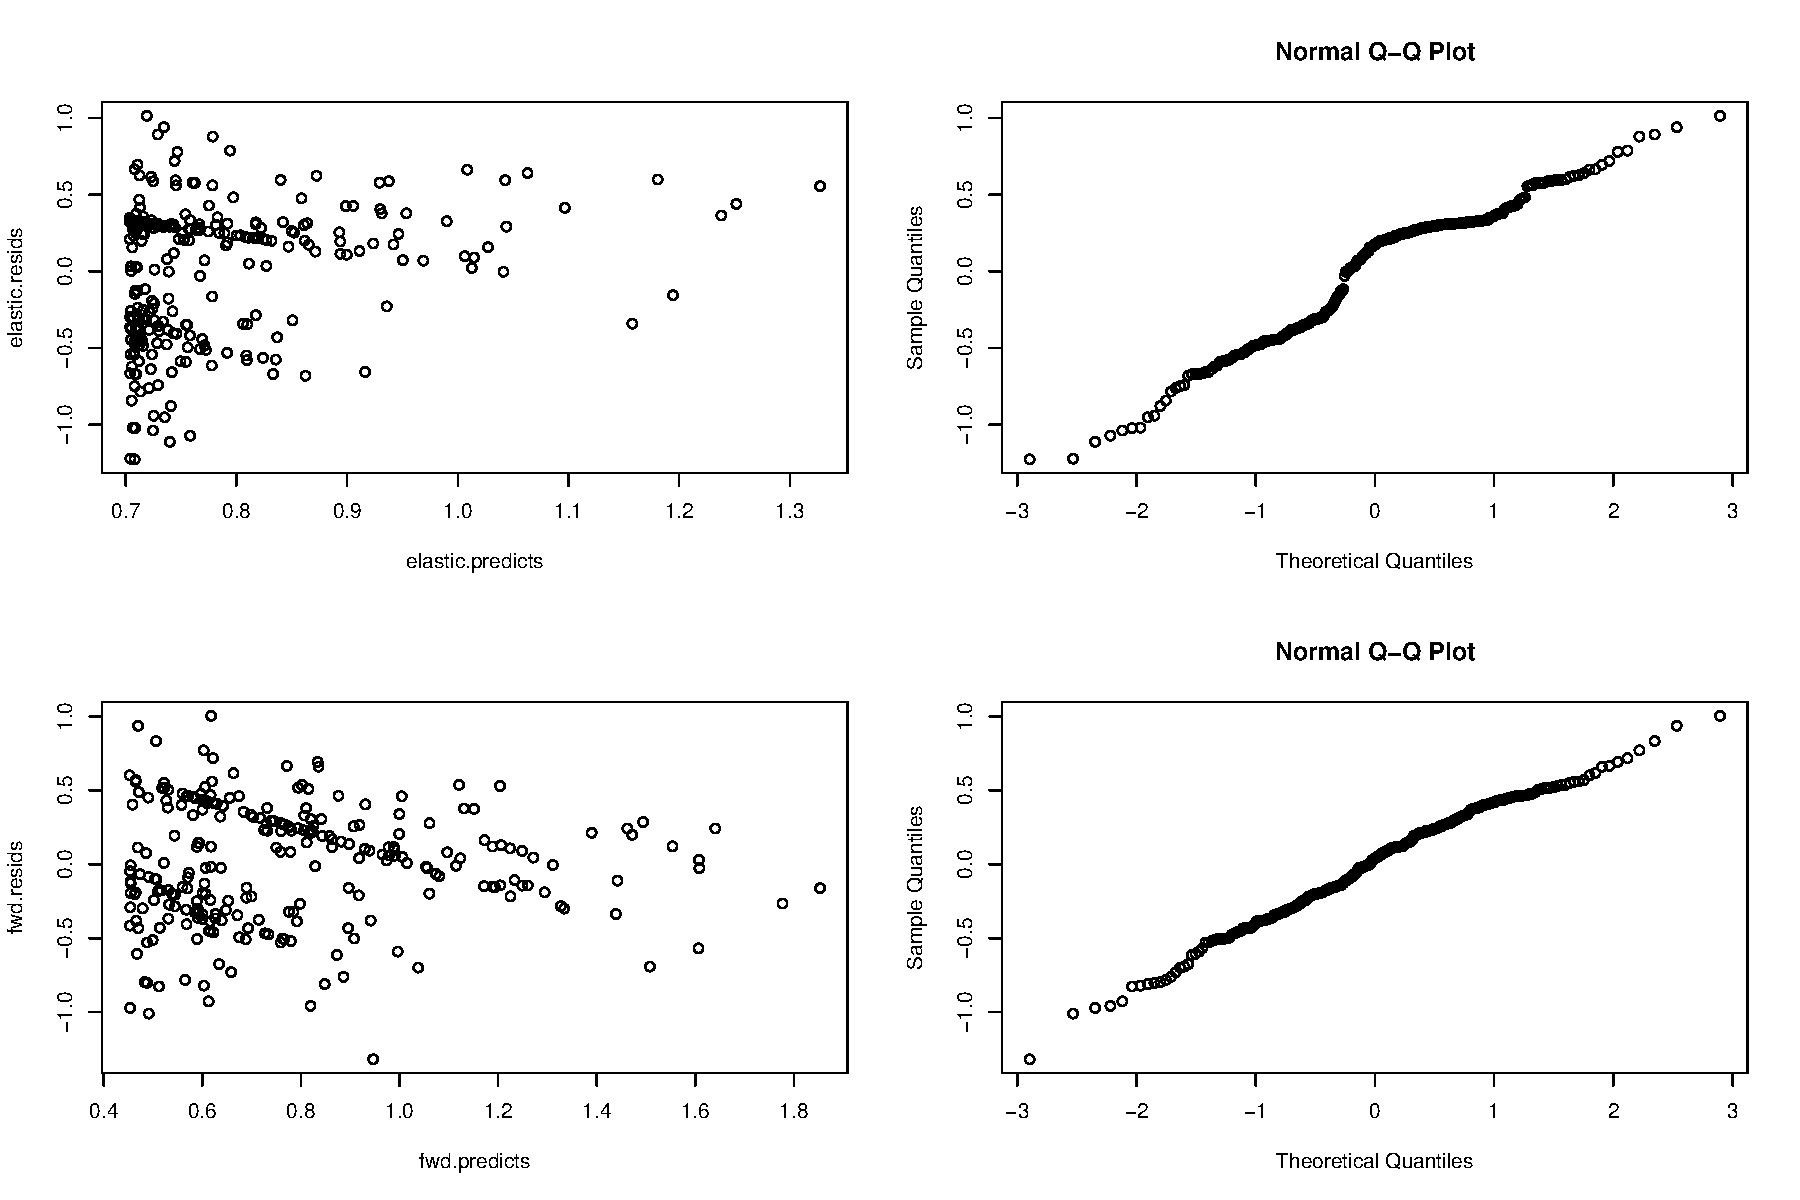
\includegraphics[width = \textwidth]{resids_workers_nonzero.pdf}
\caption{Diagnostic Residual plots for Nonzero workers.}
\label{figure:resids_workers_nonzero}
\end{figure}

\begin{table}[h!]
\begin{tabular}{l|c|c}\hline%
\bfseries \underline{Variable} & \bfseries \underline{Elasticnet} & \bfseries \underline{Forward~Selection}
\csvreader[head to column names]{fullcoeflist_invasive_binary.csv}{}%
{\\\variable & \elastic & \forward}%
\\\hline
\end{tabular}
\caption{Full coefficient list for Binary Invasive model}
\label{table:workers_invasive_full}
\end{table}

\begin{table}[h!]
\begin{tabular}{l|c|c}\hline%
\bfseries \underline{Variable} & \bfseries \underline{Elasticnet} & \bfseries \underline{Forward~Selection}
\csvreader[head to column names]{fullcoeflist_invasive_nonzero.csv}{}%
{\\\variable & \elastic & \forward}%
\\\hline
\end{tabular}
\caption{Full coefficient list for Nonzero Invasive model}
\label{table:invasive_nonzero_full}
\end{table}

\begin{figure}[h]
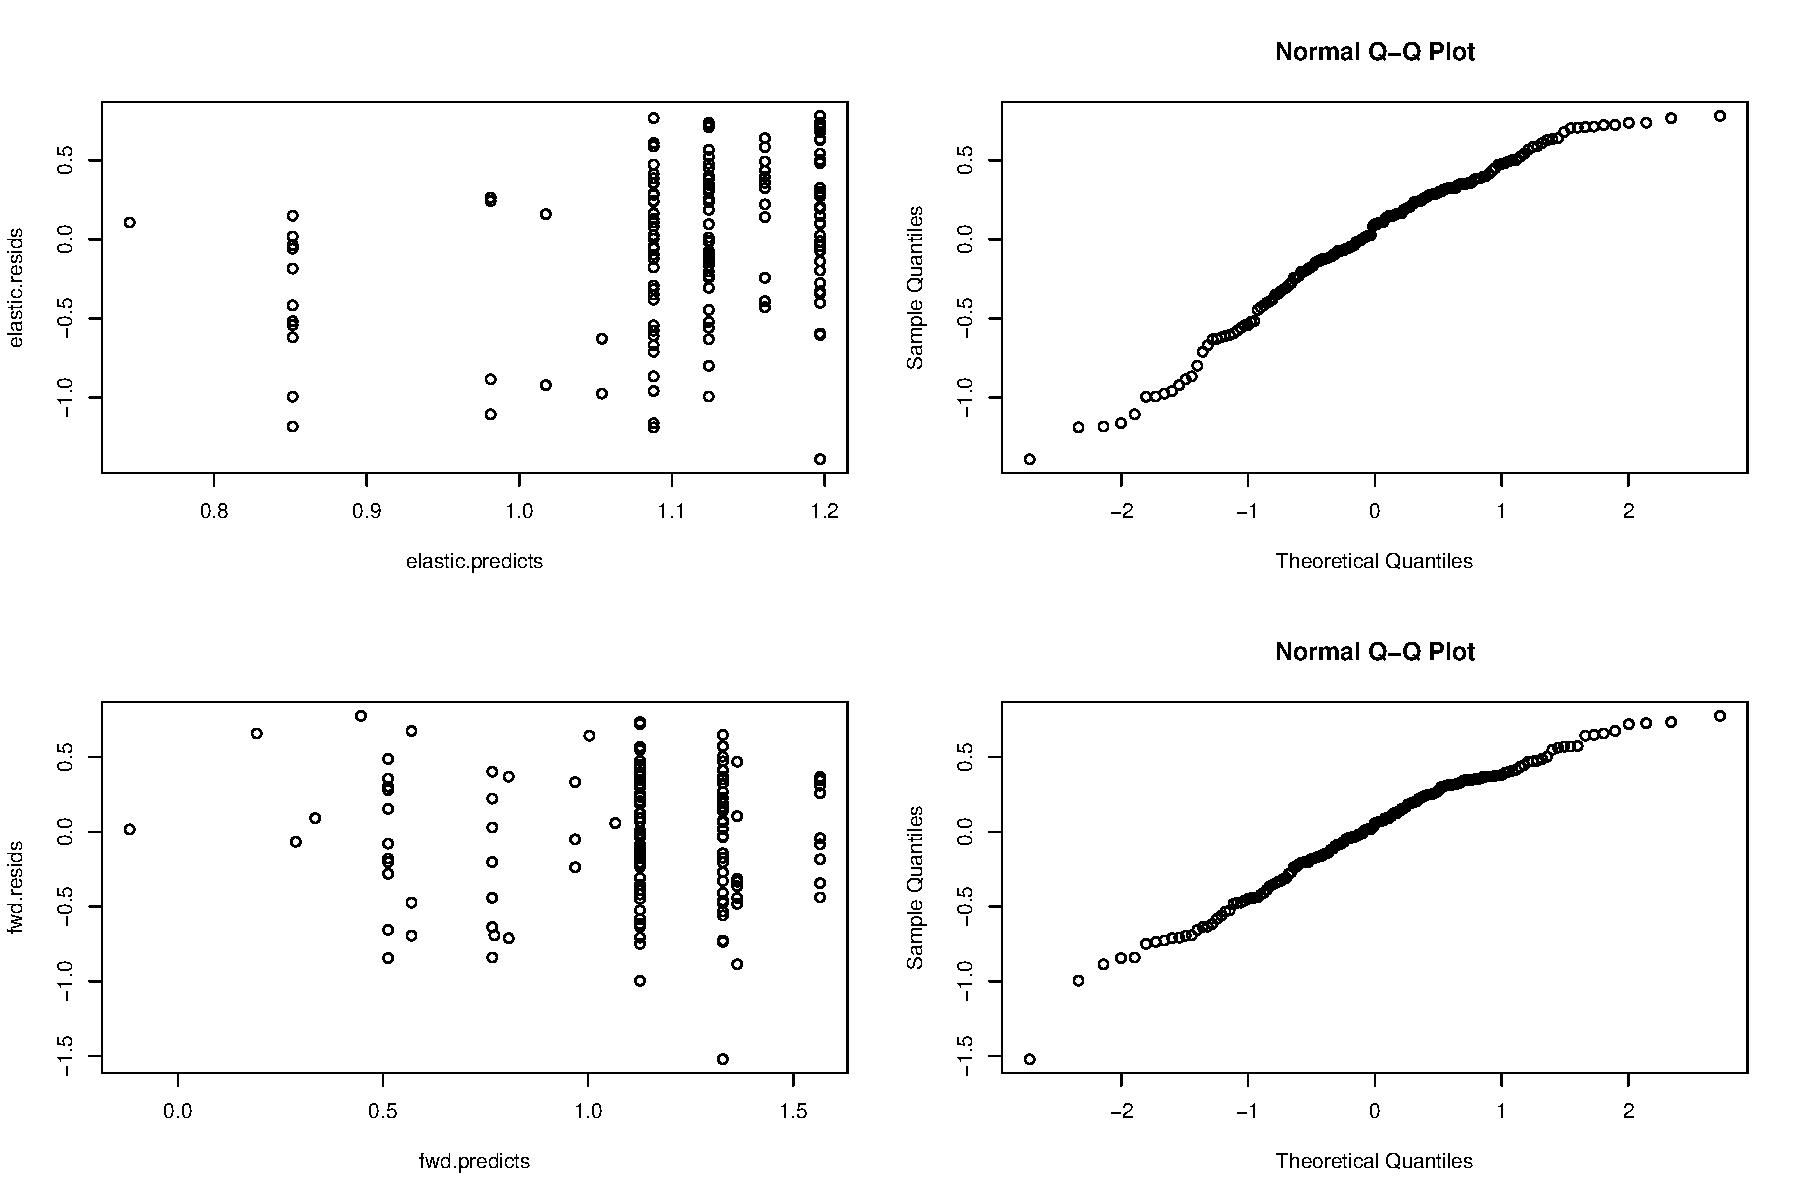
\includegraphics[width = \textwidth]{resids_invasive_nonzero.pdf}
\caption{Diagnostic Residual plots for Nonzero Invasive.}
\label{figure:resids_invasive_nonzero}
\end{figure}

\end{document}



